\documentclass[english]{article}
\usepackage{misc/style, misc/macros, misc/quiver}
\usepackage{showlabels}
\addbibresource{misc/sources.bib}

\title{Revisiting topological fixed point theory}
\author{Oscar Harr \and Florian Riedel}

\begin{document}

\maketitle

\tableofcontents

\section{Fixed point theory and six-functor formalisms}
% Throughout this section, unless otherwise specified, we fix a 
% locally rigid category $\cA$, a geometric setup $(\cC,\cE)$ in 
% the sense of \cref{defn: geometric setup}
% and an $\cA$-linear six functor formalism
% \[ \cD \colon\Span{\cC}_{\cE}\longrightarrow \pPrl{\cA} \]
% in the sense of~\cite[App~A.5]{Mann2022}. We assume for simplicity that $\cC$ contains all finite limits, so that $\cD $ is a lax symmetric monoidal functor, where $\Span{\cC}_{\cE}$ is equipped with the symmetric monoidal structure described in~\cite[Rem~A.5.5]{Mann2022}. 
% It follows formally that $\cD '(\pt )$ has a canonical commutative algebra structure and that $\cD '$ factors through a symmetric monoidal functor
% \[
%   \cD\colon\Span{\cC}_{\cE}\longrightarrow\pPrl{\cD '(\pt )}.
% \]
% (Note that $\cD (X)$ has the same underlying presentable stable $\infty$-category as $\cD '(X)$.) We will assume the following:
% Crucially, we also assume that:
% \begin{enumerate}[label=(\Alph*)]
% \item\label{monoidality-assumption} The functor $\cD$ is symmetric
%     monoidal.
% \end{enumerate}

% In particular, this means that $\D(\pt)=\cA$ and the natural comparison map
%   \[
%     \cD (X)\otimes_{\cA}\cD (Y)\longrightarrow\cD(X\times Y)
%   \]
%   is an equivalence for each pair of objects $X$ and $Y$ in $\cC$.

Assumption~\labelcref{monoidality-assumption} is satisfied for the six-functor formalisms that interest us in this paper, such as the six-functor of sheaves of on locally compact Hausdorff spaces and of local systems on anima.\Onote{Find reference for the fact that it fails for \'etale sheaves}


\subsection{The categorified Lefschetz trace formula}

Throughout this section, we put ourselves in the following:

\begin{set}
Let $(\cC,\cE)$ be a geometric context and write $\Span{\cC}_{\cE}$ for the
associated $(\infty,1)$ category of spans. Moreover, let $\cA$ be a locally
rigid $\infty$-category and fix a symmetric monoidal
functor
\[ \cD\colon \Span{\cC}_{\cE}\too \pPrl{\cA}\,.\]
\end{set}

The starting point is the following observation about dualizable
objects in span categories:

\begin{lem}\label{lem: Duality in Span}
If $X\in \cC$ is admissible,
  then $X \in \Span{\cC}_{\cE}$ is self-dual (and in particular dualizable), with evaluation and unit given by the spans
  \[X\xleftarrow{\id} X \xrightarrow{\Delta} X\times X\,, \quad
    \pt \xleftarrow{} X \xrightarrow{\id} X\,\]
  respectively, and counit and coevaluation given by the flipped spans.
\end{lem}

\begin{defn}\label{defn: coincidence locus}
    For any span $\Lambda=\left(Y\xleftarrow{g}X \xrightarrow{f} Y\right)\in \Span{\cC}_{\cE}$ we define its \tdef{coincidence locus}
    of $\Lambda$ is as the pullback:
  \begin{equation}
    \label{eq:pullback-defn-of-fixedpts}
    \begin{tikzcd}
      \mdef{X^{\Lambda}}  & Y \\
      X & Y\times Y\,.
      \arrow[from=1-1, to=1-2]
      \arrow["\lrcorner",phantom,very near start, from=1-1, to=2-2]
      \arrow[from=1-1, to=2-1]
      \arrow["\Delta", from=1-2, to=2-2]
      \arrow["{(g ,f)}"', from=2-1, to=2-2]
    \end{tikzcd}
  \end{equation}
  If $X=Y$ and $g=\id$, we also write $X^{\Lambda}=X^f$ and refer
  to it as the \tdef{fixed point locus} of $f$, and vice versa for $g$. 
\end{defn}

\begin{lem}\label{lem: trace in Span}
For any $\Lambda=\left(Y\xleftarrow{g}X \xrightarrow{f} Y\right)\in \Span{\cC}_{\cE}$ with $X,Y\in \cC$ admissible, the trace of $\Lambda$ 
   is given by the coincidence locus, i.e.~we have:
   \[ \tr{\Lambda}{\Span{\cC,\cE}} \simeq \left(\pt \leftarrow X^{\Lambda} \rightarrow \pt \right) \in \Map_{\Span{\cC}_{\cE}} (\pt, \pt)\]
\end{lem}
\begin{proof}
    Using the description of the evaluation and coevaluation on $X$ from 
  \cref{lem: Duality in Span}, we then find that the trace of the
 $\Lambda$ is given by the outer span in the diagram:
  \begin{equation}
    \label{eq:trace-in-span-category}
    \begin{tikzpicture}[baseline=(current bounding box.center),scale=2]
      %%% Nodes
      % bottom row (R0)
      \node (R0C0) at (-3,0){$\pt$};
      \node (R0C2) at (-1,0){$X\times X$};
      \node (R0C4) at (1,0){$X\times X$};
      \node (R0C6) at (3,0){$\pt$,};

      % R1
      \node (R1C1) at (-2,1){$X$};
      \node (R1C3) at (0,1){$X\times X$};
      \node (R1C5) at (2,1){$X$};

      % R2
      \node (R2C2) at (-1,2){$P$};
      \node[rotate=-45] (pullback1) at (-1,1.7){{\large $\lrcorner$}};
      \node (R2C4) at (1,2){$X$};
      \node[rotate=-45] (pullback1) at (1,1.7){{\large $\lrcorner$}};

      % R3
      \node (R3C3) at (0,3){$P^{\prime}$};
      \node[rotate=-45] (pullback1) at (0,2.7){{\large $\lrcorner$}};

      %%% Edges
      % Towards left
      \draw
      (R3C3) edge[->] (R2C2)
      (R2C2) edge[->] (R1C1)
      (R1C1) edge[->] (R0C0);

      \draw (R2C4) edge[->] node[near start,left=3pt]{{\small $\Delta$}} (R1C3)
      (R1C3) edge[->] node[near start ,left=3pt]{{\small $f\times\id$}} (R0C2);

      \draw (R1C5) edge[->] node[near start,left=3pt]{{\small $\Delta$}} (R0C4);

      % Towards right
      \draw
      (R3C3) edge[->] (R2C4)
      (R2C4) edge[double distance=1.5pt] (R1C5)
      (R1C5) edge[->] (R0C6);

      \draw
      (R2C2) edge[->] (R1C3)
      (R1C3) edge[double distance=1.5pt] (R0C4);

      \draw (R1C1) edge[->] node[near start,right=3pt]{{\small $\Delta$}} (R0C2);
    \end{tikzpicture}
  \end{equation}
  where by the pasting law the top corner $P'$ can be computed as the pullback~\eqref{eq:pullback-defn-of-fixedpts}, i.e. there is a canonical equivalence $P'\simeq X^f$. Note also that $X^f$ is separated since $X^f\to X$ is pulled back from $\Delta\colon X\to X\times X$ and thus admissible, whence the composition $X^f\to X\to\pt$ is admissible.
\end{proof}
% We assume further that
% \begin{itemize}
% \item[(M)]\label{ass: monoidal} The lax symmetric monoidal structure on $\mathcal D\colon\Span{\mathcal C}_{\mathcal E}\to\mathrm{Pr}^{\mathrm{L}}_{\mathcal A}$ exhibits $\mathcal D$ as a (strong) symmetric monoidal functor.
% \end{itemize}
% We also fix an object $X\in\mathcal C$, and assume that
% \begin{itemize}
% \item[(S)]\label{ass: seperated} The projection to the terminal object $X\to\pt$ is admissible.
% \end{itemize}
% We refer to an object satisfying (S) as \tdef{separated}.
% \\
% Since admissible morphisms are stable under base-change, the diagonal morphism $\Delta\colon X\to X\times X$ of a separated object is also admissible. This implies that $X$ is self-dual as an object of $\Span{\mathcal C}_{\mathcal E}$ \todo{REF, universality of spans?}, 
% \[
%   \begin{tikzpicture}[baseline=(current bounding box.center)]
%     \node (X) at (0,1){$X$};
%     \node (pt) at (-1,0){$\pt $};
%     \node (XX) at (1,0){$X\times X$};

%     \draw (X) edge[->] (pt);
%     \draw (X) edge[->] node[very near start,right=3pt]{{\small $\Delta$}}(XX);
%   \end{tikzpicture}
%   \qquad\text{and}\qquad
%   \begin{tikzpicture}[baseline=(current bounding box.center)]
%     \node (X) at (0,1){$X$};
%     \node (pt) at (1,0){$X .$};
%     \node (XX) at (-1,0){$X\times X$};

%     \draw (X) edge[->] (pt);
%     \draw (X) edge[->] node[very near start,left=3pt]{{\small $\Delta$}}(XX);
%   \end{tikzpicture}
% \]

% Using our assumption~\labelcref{monoidality-assumption}, we deduce that $\cD (X)$ is dualizable as an object of $\pPrl{\cA}$ for each admissible $X\in\cC$. In particular, for an endofunctor $F\colon\cD (X)\to\cD (X)$, we can take the trace $\tr{F\curvearrowright\cD (X)}{\pPrl{\cA}}$. 
% The first incarnation of the Lefschetz trace formula that we consider is a description of this trace when $F$ is a pullback functor $f^*$ for some endomorphism $f\curvearrowright X$ in $\cC$.
% Now let $\cA$ be some locally rigid $\infty$-category and let
% $\cD\colon \Span{\cC; \all, \cE}\to \pPrl{\cA}$ be some symmetric monoidal
% $\cA$-linear six functor formalism. Then \cref{lem: Duality in Span} tells
% us that, for any admissible $X\in \cC$, the category $\D{X}\in \pPrl{\cA}$
% is also dualizable and self dual. Moreover, we can compute
% the trace of any functor $F\colon \D{X}\to \D{X}$ induced by some
% span in $\Span(\cC,\all,\cE)$ as follows:

\begin{prop}[Categorified trace formula]\label{thm:categorical-fixed-pts}
% Let $\cD\colon \Span{\cC}_{\cE}\to \pPrl{\cA}$ be a symmetric monoidal,
% $\cA$-linear six-functor formalism and 
Let $\cA$ be a locally rigid category and $\cD\colon \Span{\cC,\cE}\to \pPrl{\cA}$ be a symmetric monoidal $\cA$-linear six functor
formalism.
For every span $\Lambda=\left(Y\xleftarrow{g}X \xrightarrow{f} Y\right)\in \Span{\cC}_{\cE}$ with $X,Y\in \cC$ admissible, we have that:
  \begin{equation}
    \label{eq:categorical-trace-formula}
    \tr{f_!g^*\colon \D{Y}\to \D{Y})}{\mathrm{Pr}^{\mathrm{L}}_{\mathcal A}}\simeq (X^\Lambda)_!(X^\Lambda)^* \in \Map_{\pPrl{\cA}}(\cA,\cA)\,.
  \end{equation}
  % If additionally $f\colon X\to X$ is admissible, we moreover have
  %   \begin{equation}
  %   \label{eq:categorical-trace-formula-exceptional}
  %   \tr{f_!\curvearrowright\mathcal D (X)}{\mathrm{Pr}^{\mathrm{L}}_{\mathcal A}}\simeq (X^f)_!(X^f)^*.
  %\end{equation}
\end{prop}
\begin{proof}
  Recall that $f_!g^*$ is by definition the result of applying 
  the functor $\cD$ to the span $\Lambda$. 
  Since $\cD$ is symmetric monoidal and so
  preserves traces by \cref{lem: sym mon preserve trace}
  we learn that the trace of $f_!g^*$ is computed by applying $\cD$ to the trace
  of $\Lambda$ computed in $\Span{\cC}_{\cE}$. Thus the claim is immediate
  from \cref{lem: trace in Span}. 
  % the symmetric monoidal functor $\mathcal D\colon \Span{\mathcal C}_{\mathcal E} \to \pPrl{\cA}$ to the span
  % \begin{equation}
  %   \label{eq:pullback-in-correspondence}
  %   \begin{tikzpicture}[baseline=(current bounding box.center)]
  %     \node (X) at (-1,0){$X$};
  %     \node (Z) at (0,1){$Y$};
  %     \node (Xprime) at (1,0){$Y,$};

  %     \draw (Z) edge[->] node[very near start,left=3.5pt]{{\footnotesize $f$}}(X);
  %     \draw (Z) edge[double equal sign distance] (Xprime);
  %   \end{tikzpicture}
  % \end{equation}
  
  % \[
  %   \begin{tikzpicture}[baseline=(current bounding box.center)]
  %     \node (X) at (0,1){$X$};
  %     \node (pt) at (-1,0){$\pt $};
  %     \node (XX) at (1,0){$X\times X$};

  %     \draw (X) edge[->] (pt);
  %     \draw (X) edge[->] node[very near start,right=3pt]{{\small $\Delta$}}(XX);
  %   \end{tikzpicture}
  %   \qquad\text{and}\qquad
  %   \begin{tikzpicture}[baseline=(current bounding box.center)]
  %     \node (X) at (0,1){$X$};
  %     \node (pt) at (1,0){$\pt $,};
  %     \node (XX) at (-1,0){$X\times X$};

  %     \draw (X) edge[->] (pt);
  %     \draw (X) edge[->] node[very near start,left=3pt]{{\small $\Delta$}}(XX);
  %   \end{tikzpicture}
  % \]
  % respectively. The trace of $X\xleftarrow{\id} X\xrightarrow{f} X$ is therefore the outer span in the diagram
  % If $f$ is admissible, the equation~\eqref{eq:categorical-trace-formula-exceptional} follows by dualizing~\eqref{eq:categorical-trace-formula}, which interchanges $({-})^*$ and $({-})_!$.
\end{proof}

\begin{rmk}\label{rmk:utopian-lefschetz}
  Note that \cref{thm:categorical-fixed-pts} looks like a utopian version of the Lefschetz trace formula from topology; it says that for any map $f\curvearrowright X$, the trace of the induced map on the categorified cohomology $\mathcal D(X)$ is isomorphic to the compactly-supported cohomology of the fixed points $X^f$. This lacks several subtleties that are present in the actual Lefschetz trace formula. For instance, the theorem neither has a transversality assumption on $f$ nor fixed point indices to correct for the lack of transversality, and there is no compactness/properness assumption on $X$. These subtleties arise from the failure of~\labelcref{eq:categorical-trace-formula} to decategorify nicely.

  Assume for simplicity that $\cA = \Sp$, as in the case of sheaves on locally compact Hausdorff spaces or local systems on anima. The naive approach to decategorification here is to apply topological Hochschild homology
  \[
    \THH\colon\Prdual\too\Sp
  \]
  on both sides of the formula. On the left-hand side, one would then want to relate $\THH$ of $\tr{f^*\curvearrowright\cD (X)}{}$ to the trace of map induced by $f$ on $\THH(\cD (X))\simeq\Gamma_c(X;\SS )$. If $\cD (X)$ were dualizable \emph{as an object of $\Prdual$}, this would be formal, since $\THH$ is symmetric monoidal and thus preserves traces of endomorphisms of dualizable objects. However, for a dualizable category to be dualizable \emph{in} dualizable categories (aka \tdef{fully dualizable} or \tdef{fully saturated}~\cite{Kontsevich2005}) is very restrictive. Indeed,~\cite{Harr2026} shows that the category of sheaves $\Shv (\tset ;\Sp )$ on a locally compact Hausdorff space $\tset$ is fully dualizable if and only if $\tset$ is a finite set of points. The failure of $\cD (X)$ to be fully dualizable also means that there is no formal reason to expect the trace of $f^*$ to be strongly continuous, even if $f^*$ is; and hence no reason for $\THH$ to even be \emph{defined} for the (equivalent) functors appearing in~\labelcref{eq:categorical-trace-formula}. Indeed, a generic self-homeomorphism of a manifold is known to have a Cantor set of fixed points~\cite{Craciun2013}, in which case the functor $(X^f)_!(X^f)^*\simeq\SS^{\oplus\aleph_0}\otimes{-}$ will fail very badly to be strongly continuous. Similar subtleties surrounding decategorification and commuting $\THH$ with trace also play a central role in~\cite{Beraldo_Pippi2024}.
\end{rmk}

\subsection{Naturality}

We now assume that the class of admissible maps $\cE$ admits a \emph{suitable decomposition}
$(\cI,\cP)$ with respect to $\cD$ in the sense of \cite[Definition A.5.9]{Mann2022}. We say that a morphism in \emph{\'etale} if it lies in $\cI$
and \emph{proper} if it lies in $\cP$.
Write $\mdef{\sSpan{\cC}_{\cE}^{\cI,\cP}}$ the
symmetric monoidal $(\infty,2)$-category of 
\cite[Definition 4.10]{Cnossen_Lenz_Linskens2026} associated to the datum
$(\cC,\cE,\cI,\cD$).\footnote{Explicitly, a non-invertible 2-cells from $X\leftarrow Z\to Y$ to  $X\leftarrow Z'\to Y$ given by a span $Z \xleftarrow{f} W\xrightarrow{i}Z'$ with $f\in \cP$ and $i\in \cI$, together with 
 homotopies making the obvious diagram commute.}
 Moreover, 
 we write $\pPrlf{\cA}$ for the $(\infty,2)$-category of presentable,
 $\cA$-linear $\infty$-categories.
% \begin{equation}\label{eq:span-of-spans}
%   \begin{tikzpicture}[baseline=(current bounding box.center)]
%     \node (X) at (-1.5,0){$X$};
%     \node (Z) at (0,1.5){$Z$};
%     \node (Zprime) at (0,-1.5){$Z',$};
%     \node (W) at (0,0){$W$};
%     \node (Y) at (1.5,0){$Y$};

%     \draw (Z) edge[->] (Y);
%     \draw (Z) edge[->] (X);
%     \draw (Zprime) edge[->] (Y);
%     \draw (Zprime) edge[->] (X);
%     \draw (W) edge[->] node[near start,left=1.5pt]{{\footnotesize $f$}}(Z);
%     \draw (W) edge[->] node[near start,left=1.5pt]{{\footnotesize $i$}}(Zprime);
%   \end{tikzpicture}
% \end{equation}
% where $i\in\cI$ and $f\in\cP$. 
% \begin{equation*}
%   \widetilde\cD'\colon\sSpan{\cC}_{\cE,\cI,\cP}^{\otimes}\too\Prlstf,
% \end{equation*}
% which on $(\infty ,1)$-categorical cores is equivalent to $\cD '$. Our assumption~\labelcref{monoidality-assumption} implies that $\widetilde\cD '$ factors through a symmetric monoidal functor
% It will useful to further analyze in which sense the 
% equivalence \labelcref{eq:categorical-trace-formula} is natural.
% The equivalence of $\labelcref{eq:categorical-trace-formula}$ a priori
% happens in the mapping \emph{space} of $\cA$-linear functors. 
% To understand the naturality in non-invertible morphisms, we need
% to upgrade $\cD$ to an $(\infty,2)$-functor. Let $\pPrlf{\cA}$ denote
% the natural $(\infty,2)$-categorical refinement of $\pPrl{\cA}$.\todo{Cite?} 
 % is a \emph{natural} equivalence in the situations that we care about. For this to make sense, we must have a functoriality in mind for both the left and right sides of the equation. This functoriality is brought to you by 2-categorical enhancements of the six-functor formalism $\cD$ \`a la \cite{Cnossen_Lenz_Linskens2026} and the higher trace machinery of~\cite{Hoyois_Scherotzke_Sibilla2017}, as we now explain.
By \cite{Cnossen_Lenz_Linskens2026} we obtain a canonical refinement
of $\cD$ to a symmetric monoidal $(\infty,2)$-functor:
\[ \mdef{\cD}\colon \sSpan{\cC}_{\cE}^{\cI,\cP}\too \pPrl{\cA}\,,\]
which we denote the same for brevity.
Then \cite[Theorem~1.7]{Hoyois_Scherotzke_Sibilla2017}
tells us that $\cD$ induces a commutative diagram of $(\infty,1)$-categories:
\begin{equation}
  \label{eq:naturality-of-lefschetz}
  \begin{tikzcd}
    \Endtrl (\sSpan{\cC}_{\cE}^{\cI,\cP}) \arrow[d,"\Trc"]\arrow[r,"\cD"]
    & \Endtrl (\pPrlf\cA )\arrow[d,"\Trc"]\\
    \Omega_{\pt} \sSpan{\cC}_{\cE}^{\cI,\cP}\arrow[r,swap, "\Omega\cD"]
    & \Omega_{\cA} \pPrlf\cA.
  \end{tikzcd}
\end{equation}
On \emph{objects} this is just the statement of \cref{lem: sym mon preserve trace} and thus allows us to recover the
equivalence~\labelcref{eq:categorical-trace-formula}.
To really leverage this, we need to understand the category 
$\Endtrl (\sSpan{\cC}_{\cE}^{\cI,\cP})$ better.
% That is, the counterclockwise composition sends a span of the form
% \[X\xleftarrow fX\xrightarrow{\id}X \]to $(X^f)_!(X^f)^*\colon\cA\to\cA$, whereas the clockwise composition spits out $\tr{f^*\curvearrowright\cD (X)}{}$. The counterclockwise resp.~clockwise composition in the diagram therefore implement the functoriality for the left-hand side resp. right-hand side of~\labelcref{eq:categorical-trace-formula}, and the invertible 2-cell filling the commutative diagram implements a natural equivalence between these functors.

% \todo{Define proper \'etale etc?}
% We already know how the clockwise composition in~\labelcref{eq:naturality-of-lefschetz} behaves on morphisms, see~\cref{sec: trace theory}. As for the counterclockwise composition, we first observe
% \Onote{actually, we dont have any use for this proposition (so maybe we should just delete it); the proposition that's actually useful is the one that comes after it.}

\begin{prop}
  Let
  \[ \Lambda =
    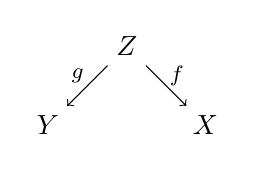
\begin{tikzpicture}[baseline=(current bounding box.center)]
      \node (X) at (1,0){$X$};
      \node (Z) at (0,1){$Z$};
      \node (Y) at (-1,0){$Y$};

      \draw (Z) edge[->] node[near start,left=1.5pt]{{\footnotesize $g$}} (Y);
      \draw (Z) edge[->] node[near start,right=1.5pt]{{\footnotesize $f$}} (X);
    \end{tikzpicture} \]
  be a 1-morphism in $\sSpan{\cC}_{\cE}^{\cI ,\cP}$ with both $f$ and $g$ admissible, and suppose that
  \begin{enumerate}[label=(\roman*)]
  \item $f$ is \'etale and the diagonal map $\Delta_f\colon Z\to Z\times_XZ$ is in proper.
  \item $g$ is proper and the diagonal map $\Delta_g\colon Z\to Z\times_YZ$ is \'etale.
  \end{enumerate}
  Then
    \[
    \Lambda '=
    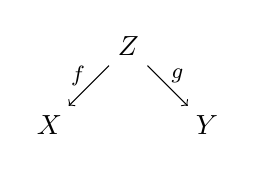
\begin{tikzpicture}[baseline=(current bounding box.center)]
      \node (X) at (-1,0){$X$};
      \node (Z) at (0,1){$Z$};
      \node (Y) at (1,0){$Y$};

      \draw (Z) edge[->] node[near start,right=1.5pt]{{\footnotesize $g$}} (Y);
      \draw (Z) edge[->] node[near start,left=1.5pt]{{\footnotesize $f$}} (X);
    \end{tikzpicture}
  \]
  is an internal right adjoint to $\Lambda$.
\end{prop}
\begin{proof}
  Note that
  \[
    \Lambda \circ\Lambda '=
    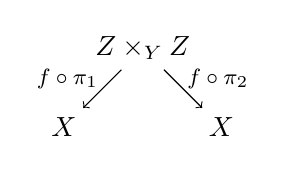
\begin{tikzpicture}[baseline=(current bounding box.center)]
      \node (X) at (1,0){$X$};
      \node (Z) at (0,1){$Z\times_YZ$};
      \node (Y) at (-1,0){$X$};

      \draw (Z) edge[->] node[near start,left=1.5pt]{{\footnotesize $f\circ\pi_1$}} (Y);
      \draw (Z) edge[->] node[near start,right=1.5pt]{{\footnotesize $f\circ\pi_2$}} (X);
    \end{tikzpicture}
    \qquad\text{and}\qquad
    \Lambda '\circ\Lambda =
    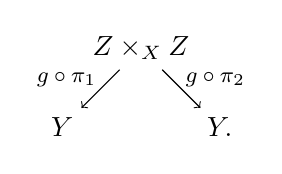
\begin{tikzpicture}[baseline=(current bounding box.center)]
      \node (X) at (1,0){$Y.$};
      \node (Z) at (0,1){$Z\times_XZ$};
      \node (Y) at (-1,0){$Y$};

      \draw (Z) edge[->] node[near start,left=1.5pt]{{\footnotesize $g\circ\pi_1$}} (Y);
      \draw (Z) edge[->] node[near start,right=1.5pt]{{\footnotesize $g\circ \pi_2$}} (X);
    \end{tikzpicture}
  \]
  By assumption, we have the following 2-morphisms in $\sSpan{\cC}_{\cE}^{\cI ,\cP}$:
  \[
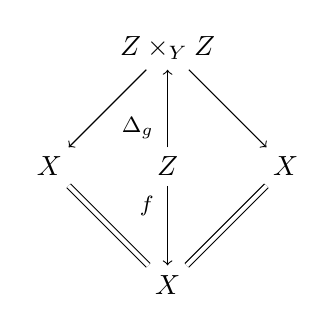
\begin{tikzpicture}[baseline=(current bounding box.center)]
    \node (X) at (-1.5,0){$X$};
    \node (Z) at (0,1.5){$Z\times_YZ$};
    \node (Zprime) at (0,-1.5){$X$};
    \node (W) at (0,0){$Z$};
    \node (Y) at (1.5,0){$X$};

    \draw (Z) edge[->] (Y);
    \draw (Z) edge[->] (X);
    \draw (Zprime) edge[double distance=1.5pt] (Y);
    \draw (Zprime) edge[double distance=1.5pt] (X);
    \draw (W) edge[->] node[near start,left=1.5pt]{{\footnotesize $\Delta_g$}}(Z);
    \draw (W) edge[->] node[near start,left=1.5pt]{{\footnotesize $f$}}(Zprime);
  \end{tikzpicture}
  \qquad\text{and}\qquad
  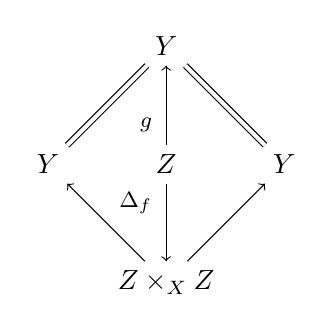
\begin{tikzpicture}[baseline=(current bounding box.center)]
    \node (X) at (-1.5,0){$Y$};
    \node (Z) at (0,-1.5){$Z\times_XZ$};
    \node (Zprime) at (0,1.5){$Y$};
    \node (W) at (0,0){$Z$};
    \node (Y) at (1.5,0){$Y$};

    \draw (Z) edge[->] (Y);
    \draw (Z) edge[->] (X);
    \draw (Zprime) edge[double distance=1.5pt] (Y);
    \draw (Zprime) edge[double distance=1.5pt] (X);
    \draw (W) edge[->] node[near start,left=1.5pt]{{\footnotesize $\Delta_f$}}(Z);
    \draw (W) edge[->] node[near start,left=1.5pt]{{\footnotesize $g$}}(Zprime);
  \end{tikzpicture}
\]
from $\Lambda \circ\Lambda '$ to $\id$ and $\id$ to $\Lambda '\circ\Lambda $, respectively. It is straightforward to check that these 2-morphisms satisfy the triangle equality, and hence witness an adjunction $\Lambda \circ\Lambda '\dashv \Lambda '\circ\Lambda$ as desired.
\end{proof}

\begin{prop}\label{prop:internal-left-adjoints}
  Let $X\in\cC$ be an admissible object.
  \begin{enumerate}[label=(\alph*)]
  \item The 1-morphism $\pt\leftarrow X\xrightarrow\id X$ has an internal right adjoint if $X$ is proper.
  \item The 1-morphism $X\xleftarrow{\id} X\to \pt$ has an internal right adjoint if $X$ is \'etale.
  \end{enumerate}
\end{prop}
\begin{proof}
  In the case of (a), there is an adjunction between $\pt\leftarrow X\xrightarrow\id X$ and $X\xleftarrow{\id} X\to \pt$ which is witnessed by the 2-morphisms
  \[
    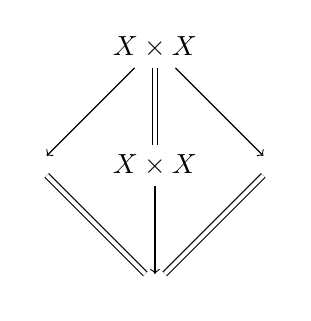
\begin{tikzpicture}[baseline=(current bounding box.center)]
      \node (X) at (-1.5,0){$\pt$};
      \node (Z) at (0,1.5){$X\times X$};
      \node (Zprime) at (0,-1.5){$\pt$};
      \node (W) at (0,0){$X\times X$};
      \node (Y) at (1.5,0){$\pt$};

      \draw (Z) edge[->] (Y);
      \draw (Z) edge[->] (X);
      \draw (Zprime) edge[double distance=1.5pt] (Y);
      \draw (Zprime) edge[double distance=1.5pt] (X);
      \draw (W) edge[double distance=1.5pt] (Z);
      \draw (W) edge[->] (Zprime);
    \end{tikzpicture}
    \qquad\text{and}\qquad
    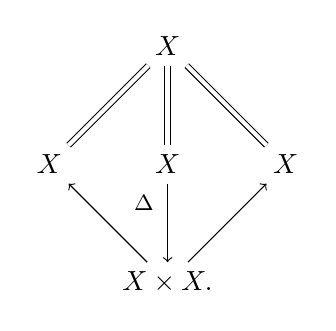
\begin{tikzpicture}[baseline=(current bounding box.center)]
      \node (X) at (-1.5,0){$X$};
      \node (Z) at (0,-1.5){$X\times X.$};
      \node (Zprime) at (0,1.5){$X$};
      \node (W) at (0,0){$X$};
      \node (Y) at (1.5,0){$X$};

      \draw (Z) edge[->] (Y);
      \draw (Z) edge[->] (X);
      \draw (Zprime) edge[double distance=1.5pt] (Y);
      \draw (Zprime) edge[double distance=1.5pt] (X);
      \draw (W) edge[->] node[near start,left=1.5pt]{{\footnotesize $\Delta$}}(Z);
      \draw (W) edge[double distance=1.5pt] (Zprime);
    \end{tikzpicture}
  \]
  As for (b), simply mirror the diagrams above along the horizontal axis.
\end{proof}
\Onote{Write that the map on traces induced by a lax comm square in span-category with internally left adjoint horizontal arrows (i.e.~a map in traceable endos) is induced by the associated map on fixed points.}

% \begin{rmk}
% Sppose that $\cD\colon \Span{\cC}_{\cE}\to \pPrl{\cA}$ is a
% symmetric monoidal six functor formalism that arises as in~\cite{Liu_Zheng2012,Mann2022} from the data of a suitable decomposition $(\cI,\cP)$ of $\cE$ \cite[Def~A.5.9]{Mann2022} and a lax symmetric monoidal functor $\cD ''\colon\cC^{\op}\to\Prlst$, such that the tuple $(\cC ,\cE ,\cI ,\cP ,\cD '')$ satisfies the conditions of~\cite[Prop~A.5.10]{Mann2022}. \cite{Cnossen_Lenz_Linskens2026} define a symmetric monoidal $(\infty ,2)$-categorical enhancement of the span category $\Span{\cC}_{\cE}$, denoted $\mdef{\sSpan{\cC}_{\cE,\cI,\cP}}$, with 2-morphismsh (See Definition 4.10 and the discussion on page 50 of op.~cit.~for a formal construction of $\sSpan{\cC}_{\cE ,\cI ,\cP}$ and its symmetric monoidal structure.) The main theorem of op.~cit. then tells us, under assumption \labelcref{monoidality-assumption}, 
% that $\cD$ refines monoidal $(\infty,2)$-functor:
% \begin{equation}
%   \label{eq:2-categorical-sixff}
%   \cD\colon\sSpan{\cC}_{\cE,\cI,\cP}\too\pPrlf\cA\,,
% \end{equation}
% which we dnote the same for brevity.
% \end{rmk}
\begin{defn}
    Given some admissible $Y,X\in \cC$, we say that an span $\Lambda=(Y\xleftarrow{g} X \xrightarrow{f}) \in \Span{\cC}_{\cE}$ is
    \tdef{$\cD$-traceable} if it satisfies the conditions of \cref{prop:internal-left-adjoints}.
\end{defn}

\subsection{Decategorification}

Following~\cite{Kondyrev_Prikhodko2020,Ben-Zvi_Nadler2021}, we decategorify~\cref{thm:categorical-fixed-pts} by using the functoriality of trace in traceable endomorphisms.

\todo{revise}
That is, for a suitable object $X\in\cC$ and a proper endomorphism $f\curvearrowright X$, we produce a commutative triangle in $\cA$ whose base implements the Lefschetz trace of $f$, and whose right leg implements fixed point indices for $f$, c.f.~\cref{rmk:utopian-lefschetz}. We will also describe a dual theory of Reidemeister traces, generalizing the classical notion of the Reidemeister trace of a self-map of an $\infty$-groupoid.

\begin{cons}\label{cons: pb tf and trc}
Let $f\colon X\to Y\in \cC$ be a morphism.
\begin{enumerate}
    \item  If $f$ is $\cD$-proper, we define the \tdef{pullback} 
        along $f$ to be the composite natural transformation
         \[ \mdef{\pb{f}}\colon Y_!Y^{\ast} \xrightarrow{\epsilon} Y_!f_{\ast}f^{\ast}Y^{\ast} = Y_!f_!f^{\ast}Y^{\ast} \simeq X_! X^{\ast}\,,\]
         where $\epsilon$ is the unit of the adjunction $f^{\ast}\dashv f_{\ast}$.
    \item If $f$ is $\cD$-\'etale, we define the \tdef{transfer}
          along $f$ to be the composite natural transformation 
          \[ \mdef{\tf{f}}\colon X_!X^{\ast}\simeq Y_!f_!f^{\ast}Y^{\ast}
          \xrightarrow{\eta} Y_!Y^{\ast}\]
          where $\eta$ is the counit of the adjunction $f_!\dashv f^{\ast}$.
    \item If $\Lambda= \left( Y \xleftarrow{g} X \xrightarrow{f} Y\right)$
          is $\cD$-traceable, the functor $Y_!Y^{\ast}$ admits an internal
          right adjoint in $\pPrlf{\cA}$ and hence the composite 
          \[  Y_!Y^{\ast} \xrightarrow{\pb{f}} X_!X^{\ast}\xrightarrow{\tf{g}} Y_!Y^\ast \]
          refines to an endomorphism of the unit $(\cA,\id)$ in
          $\Endtrl(\pPrlf{\cA})$. We define the $\cA$-linear trace 
  \[ \mdef{\tr{\Lambda}{\cA}} \colon \1_{\cA} \to \1_{\cA} \]
  as the image of this morphism under the symmetric monoidal functor 
  $\Trc\colon \Endtrl(\pPrlf{\cA})\to \Omega\cA$ of REF. 
    \end{enumerate}
\end{cons}

\begin{rmk}\label{rmk: about pb tf and trc}
Some remarks:\todo{Finish this rmk}
    \begin{enumerate}
        \item What happens when one of the legs is identity.
        \item If $\1_\cA\in \cA^{\omega}$ then $X_!X^{\ast}\1_{\cA}$
        is dualizable and $\tr{\pb{f}}{\cA}$ is actually the trace
        of $\pb{f}(\1_\cA)$. 
        \item This is precisely the Lefschetz trace.
    \end{enumerate}
\end{rmk}

\begin{prop}\label{prop: coincidence triangle}
    For any $\cD$-traceable span $\Lambda= \left( Y \xleftarrow{g} X \xrightarrow{f} Y\right)$ with coincidence locus $X^{\Lambda}$, 
    we have a commutative diagram:
    \begin{equation}\label{eq: coincidence triangle}
    \begin{tikzcd}[column sep=small]
      & (X^\Lambda)_!(X^\Lambda)^*\1_{\cA} \arrow[dr]\\
      \1_{\cA}\arrow[rr,swap,"\tr{\Lambda}{\cA}"]\arrow[ru] & & \mathbf \1_{\cA}\,.
    \end{tikzcd}
    \end{equation}
   Additionally, in the case that $X=Y$, the following are true:
   \begin{enumerate}
       \item If $g= \id$, then the map $\1_{\cA}\to (X^{\Lambda})_!(X^{\Lambda})^{\ast}\1_{\cA}$ naturally identifies with the
       unit map $\1_{\cA}\to (X^f)_!(X^f)^{\ast}\1_{\cA}$.
       \item If $f=\id$, then the map $(X^{\Lambda})_!(X^{\Lambda})^{\ast}\1_{\cA}\to \1_{\cA}$ naturally identifies
       with the counit map $(X^g)_!(X^g)^{\ast}\1_{\cA}\to \1_{\cA}$
   \end{enumerate}
\end{prop}
\begin{proof}
   Indeed, the morphism $\tf{g}\pb{f}$ factors in $\Endtrl(\pPrlf{\cA})$
   as:
   \[
  \begin{tikzcd}
	\cA & {\D{Y}} & \cA \\
	\cA & {\D{Y}} & \cA
	\arrow["{Y^{\ast}}", from=1-1, to=1-2]
	\arrow[equals, from=1-1, to=2-1]
	\arrow["{Y_!}", from=1-2, to=1-3]
	\arrow["{f_!g^{\ast}}", from=1-2, to=2-2]
	\arrow[equals, from=1-3, to=2-3]
	\arrow[Rightarrow, from=2-1, to=1-2]
	\arrow["{Y^{\ast}}"', from=2-1, to=2-2]
	\arrow[Rightarrow, from=2-2, to=1-3]
	\arrow["{Y_!}"', from=2-2, to=2-3]
\end{tikzcd} 
\]
where the left hand two-cell is given by the composite
\[ Y^{*} \xrightarrow{\epsilon} g_{*}g^{*} Y^{*} =g_!g^{*}Y^* \simeq g_!X^*
 \simeq g_! f^* Y^*\,, \]
 and the right hand two-cell is the composite
 \[ Y_! f_!g^* \simeq X_!g^{*} \simeq Y_!g_!g^*= Y_!g_{\sharp}g^*
 \xrightarrow{\eta} Y_!\,.\]
Applying the functor $\TrcL$, we obtain the desired factorization
from the identification $\TrcL(f_!g^*)\simeq (X^{\Lambda})_!(X^{\Lambda})^{\ast}$ of \todo{Add REF in correct generality}. 

If $X=Y$ and $g=\id$, the right-hand square is the image of the morphism
  \[
    \begin{tikzcd}
      \pt\arrow[r,leftarrow]\arrow[dd,equal]
      & X\arrow[r,equal]
      & X\arrow[d,equal]\\
       & & X \arrow[d,"f"]\\
      \pt\arrow[r,leftarrow]
      & X\arrow[r,equal]
      & X
    \end{tikzcd}
  \]
  in $\Endtrl (\sSpan{\cC}_{\cE,\cI,\cP})$ by~\cref{prop:internal-left-adjoints}, and it follows from the commutativity of~\labelcref{eq:naturality-of-lefschetz} that the induced map on traces is induced by the projection $X^f\to\pt$. The case of $f=\id$ is completely
  analogous.
\end{proof}

\begin{defn}\label{defn: characters}
    Let $\Lambda=\left( X= X \xrightarrow{f} X\right)$ and
    $\Lambda^{\prime} = \left(Y\xleftarrow{g} Y =Y\right)$ be two 
    $\cD$-traceable spans. 
    We define the \tdef{Lefschetz character} of $f$ as the morphism 
    \[ \mdef{\lambda_f}\colon (X^f)_!(X^f)^*\1_{\cA}\to \1_{\cA} \]
    given by the right hand diagonal map in \eqref{eq: coincidence triangle}. 
    Moreover, we define the \tdef{Reidemeister character} of $g$ as
    the morphism
    \[ \mdef{\rho_g}\colon \1_{\cA}\to (Y^g)_!(Y^g)^*\1_{\cA}\]
    given by the left hand diagonal map in \eqref{eq: coincidence triangle}.
\end{defn}

\begin{war}
    Something about the terminology goes here \todo{Write it}.
\end{war}

\begin{exam}
    The extreme case where $f=g=\id$ tells us something
    about the Euler characteristic \todo{Maybe remark this later?}
\end{exam}

%\subsubsection{Lefschetz}

% \begin{cons}
% Let $X \in \cC$ be suave and prim and let $f\colon X\to X$
% be a self map that is cohomologically proper. 
% Then the functor $X_!X^{\ast}\colon \cA\to \cA$
% is strongly continuous and hence the pullback 
% $\pb{f}\colon X_!X^{\ast}\to X_!X^{\ast}$ along
% $f$ defines a morphism
%   \begin{equation}
%     \label{eq:abstract-lefschetz-trace}
%     \begin{tikzcd}[column sep=huge]
%       \cA \arrow[d,equal] \arrow[r,"X_!X^*"] & \cA\arrow[d,equal]\\
%       \cA \arrow[r,swap, "X_!X^*"] \arrow[ru,Rightarrow, shorten <=15pt,shorten >=15pt ,"\pb{f}"] & \cA
%     \end{tikzcd}
%   \end{equation}
%   in the category $\Endtrl (\pPrlf\cA )$. Applying the symmetric monoidal functor 
%   $\Trc\colon \Endtrl (\pPrlf\cA ) \to \Omega_{\1_{\cA}}\cA$ of REF,
%   we obtain an endomorphism which we denote:
%   \[ \mdef{\tr{\pb{f}}{\cA}}\colon \1_{\cA}\to \1_{\cA}\,.\]
% \end{cons} 


%  The trick to factoring the map $\tr{\pb{f}}{\cA}$
%  to factor the map $(\pb{f}, X_!X^{\ast})$ in the category 
%  $\Endtrl(\pPrlf{\cA})$.
   
% \begin{prop}[The Lefschetz trace formula]\label{prop:lefschetz-trace}
%   Suppose that $X\in\cC$ is suave and prim and that $f\curvearrowright X$ is a cohomologically proper endomorphism. There is a commutative diagram
%   \begin{equation}
%     \label{eq:abstract-lefschetz-triangle}
%     \begin{tikzcd}[column sep=small]
%       & (X^f)_!(X^f)^*\mathbf 1\arrow[dr]\\
%       \mathbf 1\arrow[rr,swap,"\ch {} f"]\arrow[ru] & & \mathbf 1.
%     \end{tikzcd}
%   \end{equation}
%   Furthermore, if $X$ is cohomologically proper, then $\mathbf 1\to (X^f)_*(X^f)^*\mathbf 1\simeq (X^f)_!(X^f)^*\mathbf 1$ is the unit of the adjunction induced by the projection $X^f\to\pt$.
% \end{prop}
% \begin{proof}
%   We can factor~\labelcref{eq:abstract-lefschetz-trace} in $\Endtrl (\pPrlf\cA )$ as the composition
%   \begin{equation}
%     \label{eq:lefschetz-square-factorization}
%     \begin{tikzcd}[column sep=huge]
%       \cA\arrow[d,equal]
%       \arrow[r,"X^*"]
%       &\cD (X)\arrow[d,"f_!"]\arrow[r,"X_!"]
%       & \cA\arrow[d,equal]\\
%       \cA\arrow[r,"X^*"]\arrow[ru,Rightarrow, shorten <=15pt,shorten >=15pt]
%       &\cD(X)\arrow[r,"X_!"]
%       & \cA,
%     \end{tikzcd}
%   \end{equation}
%   where the 2-cell in the left-hand square is $X^*\xrightarrow{\mathrm{unit}} f_!f^*X^*\simeq f_!X^*$.  Applying $\TrcL$ to the composition~\labelcref{eq:lefschetz-square-factorization} and invoking~\cref{thm:categorical-fixed-pts}, we get~\labelcref{eq:abstract-lefschetz-triangle}. If $X$ is cohomologically proper, the right-hand square is the image of the morphism
%   \[
%     \begin{tikzcd}
%       \pt\arrow[r,leftarrow]\arrow[dd,equal]
%       & X\arrow[r,equal]
%       & X\arrow[d,equal]\\
%        & & X \arrow[d,"f"]\\
%       \pt\arrow[r,leftarrow]
%       & X\arrow[r,equal]
%       & X
%     \end{tikzcd}
%   \]
%   in $\Endtrl (\sSpan{\cC}_{\cE,\cI,\cP})$ by~\cref{prop:internal-left-adjoints}, and it follows from the commutativity of~\labelcref{eq:naturality-of-lefschetz} that the induced map on traces is induced by the projection $X^f\to\pt$.
% \end{proof}
%   \begin{defn}
%   Let $f\curvearrowright X$ be as in the preceding proposition. The map $(X^f)_!(X^f)^*\mathbf 1\to\mathbf 1$ from~\labelcref{eq:abstract-lefschetz-triangle} is called the \tdef{Lefschetz character} of $f$.
% \end{defn}

  
% \subsubsection{Reidemeister}

% \begin{cons}
%   Suppose that $X\in\cC$ is suave and prim and that $f\colon X\to X$
%   is a cohomologically \'etale endomorphism. Then the transfer
%   along $f$ defines a morphism
%   \begin{equation}
%     \label{eq:abstract-prereidemeister-trace}
%     \begin{tikzcd}[column sep=huge]
%       \cA\arrow[d,equal] \arrow[r,"X_!X^*"] & \cA\arrow[d,equal]\\
%       \cA\arrow[r,swap,"X_!X^*"]\arrow[ru,Rightarrow, shorten <=15pt,shorten >=15pt ,"\tf{f}"] & \cA
%     \end{tikzcd}
%   \end{equation}
%   in $\Endtrl (\pPrlf\cA )$. Applying the 
  
%   % The \tdef{Reidemeister trace} of a cohomologically \'etale endomorphism $f\curvearrowright X$, denoted $\mdef{\chr{}{f}}$, is the $\cA$-linear trace of the induced morphism
% \end{cons}

% \begin{war}
%   Usually, the term ``Reidemeister trace'' refers to a map $\mathbf 1\to (X^f)_!(X^f)^*\mathbf 1$. This is not what we are calling the Reidemeister trace. In order to emphasize the parallels with the previous subsection, we will instead refer to the classical invariant as a character
% \end{war}

% \begin{prop}\label{prop:reidemeister-trace}
%     Suppose that $X\in\cC$ is suave and prim and that $f\curvearrowright X$ is a cohomologically \'etale endomorphism. There is a commutative diagram
%   \begin{equation}
%     \label{eq:abstract-reidemeister-triangle}
%     \begin{tikzcd}[column sep=small]
%       & (X^f)_!(X^f)^*\mathbf 1\arrow[dr]\\
%       \mathbf 1\arrow[rr,swap,"\chr {} f"]\arrow[ru] & & \mathbf 1.
%     \end{tikzcd}
%   \end{equation}
%   Furthermore, if $X$ is cohomologically \'etale, then $(X^f)_!(X^f)^*\mathbf 1\simeq (X^f)_!(X^f)^!\mathbf 1\to\mathbf 1$ is the unit of the adjunction induced by the projection $X^f\to\pt$.
% \end{prop}
% \begin{proof}
%   The proof is analogous to the proof of~\cref{prop:lefschetz-trace}, using the factorization
%   \begin{equation}
%     \label{eq:lefschetz-square-factorization}
%     \begin{tikzcd}[column sep=huge]
%       \cA\arrow[d,equal]
%       \arrow[r,"X^*"]
%       &\cD (X)\arrow[d,"f^*"]\arrow[r,"X_!"]
%       & \cA\arrow[d,equal]\\
%       \cA\arrow[r,"X^*"]
%       &\cD(X)\arrow[r,"X_!"]\arrow[ru,Rightarrow, shorten <=15pt,shorten >=15pt]
%       & \cA,
%     \end{tikzcd}
%   \end{equation}
%   of~\labelcref{eq:abstract-prereidemeister-trace}.
% \end{proof}
% \begin{defn}
%   Let $f\curvearrowright X$ be as in the preceding proposition. We refer to the map $\mathbf 1\to (X^f)_!(X^f)^*\mathbf 1$ from~\labelcref{eq:abstract-reidemeister-triangle} as the \tdef{Reidemeister cocharacter} of $f$.
% \end{defn}

%%% Local Variables:
%%% mode: LaTeX
%%% TeX-master: "main"
%%% End:


\section{Deducing Lefschetz theorems in topology}\label{sec:lefschetz}
% \subsection{Local systems and the Reidemeister trace}

% Let $g\colon \anima\to \anima$ be a self-map of a compact anima $\anima$. Consider again the lax commutative square~\eqref{eq:lax-comm-square-lefschetz} from~\cref{sec: lefschetz theory}, which we viewed as a morphism in the category of traceable endomorphisms $\Endtrl(\Prlstf)$. If $g\colon \anima\to \anima$ happened to be induced by a self-map $f\colon\tset\to\tset$ for some well-behaved space $\tset$, we recovered the Lefschetz fixed point theorem for $f$ by factoring~\eqref{eq:lax-comm-square-lefschetz} through the object $(\D{\tset },f_!)\in\Endtrl(\Prlstf)$.

% Putting topology aside for now, a more obvious factorization of~\eqref{eq:lax-comm-square-lefschetz} is through the category of local systems (aka parametrized spectra) $\Sp^\anima$:
% \begin{prop}
%   Let $g\colon \anima\to \anima$ be a self-map of a compact anima $\anima$. Considered as a morphism in $\Endtrl(\Prlstf)$, the lax commutative square~\eqref{eq:lax-comm-square-lefschetz} factors as
%   \begin{equation}\label{eq:lax-composition-reidemeister}
% \begin{tikzcd}
% 	\Sp & {\Sp^{\anima}} & \Sp \\
% 	\Sp & {\Sp^{\anima}} & \Sp
% 	\arrow["{\anima^{\ast}}", from=1-1, to=1-2]
% 	\arrow["\id"', from=1-1, to=2-1]
% 	\arrow["{\anima_\sharp}", from=1-2, to=1-3]
% 	\arrow["{g^{\ast}}", from=1-2, to=2-2]
% 	\arrow["\id", from=1-3, to=2-3]
% 	\arrow[Rightarrow, from=2-2, to=1-3]
% 	\arrow["{\anima^{\ast}}"', from=2-1, to=2-2]
%     \arrow[Rightarrow, from=2-1, to=1-2]
% 	\arrow["{\anima_{\sharp}}"', from=2-2, to=2-3]
% \end{tikzcd}
%     % \left(
%     %   \begin{tikzcd}[column sep=large]
%     %     \Sp^X \arrow[r,"X_\sharp"] \arrow[d,"g^*"] & \Sp \arrow[d,equal]\\
%     %     \Sp^X \arrow[r,swap,"X_\sharp"]  \arrow[ru,Rightarrow, shorten <=5pt,shorten >=5pt]  & \Sp
%     %   \end{tikzcd}
%     % \right)
%     % \circ
%     % \left(
%     %   \begin{tikzcd}[column sep=large]
%     %     \Sp \arrow[r,"X^*"] \arrow[d,equal] & \Sp^X \arrow[d,"g^*"]\\
%     %     \Sp \arrow[r,swap,"X^*"] & \Sp^X
%     %   \end{tikzcd}
%     % \right),
%   \end{equation}
%   where the left hand $2$-cell is the invertible one coming from functoriality of pullback, and the right hand $2$-cell is the counit transformation $\anima_\sharp g^*\simeq \anima_\sharp g_\sharp g^*\to \anima_\sharp$.
% \end{prop}
% \begin{proof}
%   Aside from the usual adjunctions $\anima_\sharp\dashv \anima^*\dashv \anima_*$, the fact that $\anima$ is compact furnishes an additional adjunction $\anima_*\dashv \Hom_{\Sp^\anima} (D_\anima,\anima^*({-}))$, where $D_\anima$ is the dualizing object of $\anima$. It follows that the horizontal morphisms in both squares are strongly continuous, and hence that they define morphisms in $\Endtrl(\Prlstf)$. Concatenating the two $2$-cells recovers the one in~\eqref{eq:lax-comm-square-lefschetz} on the nose.
% \end{proof}
% As in the previous section, we then get
% \begin{cor}\label{cor: reidemeister lefschetz triangle}
%   For a self-map $g\colon \anima\to \anima$ of a compact anima $\anima$, there is a commutative diagram
%   \begin{equation}
%     \label{eq:reidemeister-lefschetz-triangle}
%     \begin{tikzcd}[column sep=tiny]
%       & \tr{g^*\curvearrowright\Sp^\anima}{}\arrow[dr] \\
%       \SS\arrow[rr]\arrow[ru] && \SS,
%     \end{tikzcd}
%   \end{equation}
%   where the bottom arrow is the Lefschetz trace of $g$.
% \end{cor}
% Just as in the previous section, the axioms of six-functor formalisms allow us to quickly compute the trace $\tr{g^*\curvearrowright\Sp^\anima}{}$ with the suspension spectrum of a space of ``fixed points'' for the map $g$. Here fixed points must be interpreted in a homotopy-invariant way; we let $\cL^g\anima$ denote the homotopical fixed point space defined to be the homotopy pullback
% \[
%   \begin{tikzcd}
%     \cL^{g}\anima  & \anima \\
%     \anima & \anima \times \anima\,.
%     \arrow[from=1-1, to=1-2]
%     \arrow["\lrcorner",phantom,very near start, from=1-1, to=2-2]
%     \arrow[from=1-1, to=2-1]
%     \arrow["\Delta", from=1-2, to=2-2]
%     \arrow["\Gamma^g"', from=2-1, to=2-2]
%   \end{tikzcd}
% \]
% That is, we have
% \begin{lem}\label{lem: reidemeister trace computation}
%   Let $g\colon \anima\to \anima$ be a self-map of a compact anima. There is an equivalence of spectra
%   \[
%     \tr{g^*\curvearrowright\Sp^\anima}{}\simeq\SS\lbrack\cL^{g}\anima\rbrack,
%   \]
%   natural in intertwining maps $h\colon (\anima,g)\to (\anima',g')$. 
% \end{lem}
% \begin{proof}
%   The identification comes about exactly as in the proof of~\cref{lem: trace computation}. Unlike in the topological setting, we do not need to require anything of $h$ beyond being an intertwining map, since any intertwining map induces a morphism
%   \begin{equation}
%     \label{eq:square-induced-by-proper-morphism}
%     \begin{tikzcd}
%       \Sp^{\anima}\arrow[r,"h_\sharp"]\arrow[d,"g^*"]
%       & \Sp^{\anima' }\arrow[d,"(g')^*"]\\
%       \Sp^{\anima}\arrow[r,"h_\sharp"]\arrow[ru,Rightarrow, shorten <=5pt,shorten >=5pt]
%       & \Sp^{\anima'}
%     \end{tikzcd}
%   \end{equation}
%   in $\Endtrl(\Prlstf)$, where the $2$-cell is the Beck--Chevalley morphism.
% \end{proof}
% Combining~\cref{lem: reidemeister trace computation} with~\cref{cor: reidemeister lefschetz triangle}, we find
% \begin{thm}
%   Let $g\colon \anima\to \anima$ be a self-map of a compact anima. There is a commutative triangle
%   \begin{equation}
%     \label{eq:reidemeister-lefschetz-triangle-with-identification}
%     \begin{tikzcd}[column sep=tiny]
%       & \SS\lbrack\cL^{g}\anima \rbrack\arrow[dr] \\
%       \SS\arrow[rr]\arrow[ru] && \SS,
%     \end{tikzcd}
%   \end{equation}
%   in which the bottom arrow is the Lefschetz trace and the arrow $\SS\lbrack\cL^{g}\anima \rbrack\to\SS$ is induced by the projection $\cL^{g}\anima \to\pt$.
% \end{thm}
% \begin{proof}
%   The second statement follows from the naturality of the identification in~\cref{lem: reidemeister trace computation}.
% \end{proof}
% We have constructed a homotopy invariant for self-maps that refines the Lefschetz trace:
% \begin{defn}
%   The map $\mdef{\rho_g}\colon \SS\to\SS\lbrack\cL^{g}\anima\rbrack$ in~\eqref{eq:reidemeister-lefschetz-triangle-with-identification} is the
%   \tdef{Reidemeister trace} of $g$.
% \end{defn}

We now apply the results of the previous section to self maps in 
topology.

\subsection{Topological fixed points}

\begin{defn}
    A \mdef{topological set} is a set $\tset$ equipped
    with a topology that is locally compact and Hausdorff. We denote
    the category of topological sets by $\Top$. 
\end{defn}

We now put ourselves in the following setting:

\begin{set}\label{set: tset}
  Consider the six-functor formalism on the geometric context
  $(\Top, \all)$ induced via the
  Liu--Zheng construction by the symmetric monoidal functor
  \[ \D{-}\colon \Top^\op \to \Prlst\,,\quad \tset \mapsto \D{\tset}=\Shv(\tset,\Sp) \]
  which sends a map $f\colon Y\to \tset$ to the pullback functor $f^*\colon\Shv (X;\Sp )\to\Shv (Y;\Sp )$. \todo{Ref Volpe?}
  By \todo{CITe } the class of all morphisms admits a suitable decomposition given by
  $(\cI ,\cP ) = (\textrm{open immersions}, \textrm{proper maps})$
  so that $\cD$ refines a to a symmetric monoidal $(\infty,2)$-functor
  \[ \cD\colon \sSpan{\Top}_{\cI,\cP}\to \Prlstf \]
  \end{set}

  Then for any $\tset \in \Top$, we have that $\tset_!\tset^* \SS= \cptSections{\tset;\SS}$
  i.e.~the spectrum $\tset_!\tset^* \SS$ is given by the
  compactly supported cohomology of the constant sheaf of spectra $\tset^*\SS$. 
  Moreover, any $\tset \in \Top$ is compact iff the map $\tset \to \pt$ is proper and any map of a compact topological sets is automatically proper. 
  In this situation, the pullback map of \cref{cons: pb tf and trc} 
  identifies with the
  classical pullback of (compactly supported) cohomology classes
  \[ \pb{f}\colon \cptSections{\tset;\SS}\to \cptSections{\tset;\SS}\,.\]
  
  Assume additionally that $\tset$ is $\cD$-suave \footnote{This holds, for instance, if $\tset$ is locally of constant shape, or more specifically if $\tset$ is an absolute neighborhood retract.}.\todo{Add REF} 
  Under these assumptions, any self map $f\colon \tset \to \tset$
  gives rise to a $\cD$-traceable span \todo{Might want to justify this}
  $\Lambda =\left(\tset= \tset \xrightarrow{f}\tset \right)$ which, as discussed
  in \cref{rmk: about pb tf and trc} has $\Sp$-linear trace simply 
  given by the symmetric monoidal trace of $\pb{f}$. 
  Moreover, \cref{prop: coincidence triangle} now supplies a commutative triangle
  \begin{equation}
    \label{eq:topological-lefschetz-trace}
    \begin{tikzcd}
      & \Gamma_c(X^f;\SS )\arrow[dr, "\lambda_f"]\\
      \SS\arrow[rr, "\tr{\pb{f}}{}"] \arrow[ru]&&\SS,
    \end{tikzcd}
  \end{equation}
  in which $\SS\to\Gamma_c(X^f;\SS )\simeq\Gamma (X^f;\SS )$ is the unit for the sheaf cohomology ring $\Gamma (X^f;\SS )\in\CAlg (\Sp)$. If $X$ is locally of constant shape, then $(\Gamma (X;\SS ),f\curvearrowright \Gamma (X;\SS ))$ is equivalent to the map induced on (singular) spherical cochains $(\SS^{\ani X},f\curvearrowright \SS^{\ani X})$. This is the usual Lefschetz trace, as one may deduce from the symmetric monoidality of the functors
  \[
    \Sp\xrightarrow{\QQ\otimes_{\SS}{-}}
    \Mod_{\QQ}\xrightarrow{\pi_*}
    \grVect_\QQ,
  \]
  where $\grVect_\QQ$ is given the Koszul rule symmetric monoidal structure. In particular, we deduce:
  
  \begin{cor}[Lefschetz fixed point theorem]
    Let $X$ be a compact Hausdorff space that is locally of constant shape, and let $f\curvearrowright X$ be some self-map. If
    \[
      \tr{\pb{f}}{} = \sum_i (-1)^i\tr{f^*\curvearrowright H^i(X;\QQ )}{}\neq 0,
    \]
    then $f$ has a fixed point.
  \end{cor}
  \begin{proof}
    If $X^f = \varnothing$ then $\Gamma_c(X^f;\SS )\simeq 0$, so commutativity of~\labelcref{eq:topological-lefschetz-trace} implies that $\tr{\pb{f}}{}\simeq 0$.
  \end{proof}
  \Onote{Maybe say something brief about fixed point indices here}

\begin{rmk}
    Suppose $X$ and $X^f$ are nice \todo{What does that mean?}. 
    Then $\lambda_f$ defines
    a class in $\pi_0\Gamma(X^f;\SS)^{\vee} \simeq H_0(X^f;\ZZ)=\ZZ[\pi_0X^f]$, i.e.~it is given by a formal sum of integers
    \[ \lambda_f= \sum_{x\in \pi_0X}[x]\lambda_f^{x}\]
    indexed by the connected components of the set of fixed points $X^f$. 
\end{rmk}
  

\subsection{Homotopy fixed points}

\begin{set}\label{set: spaces}
Consider the six-functor formalism of parametrized spectra on the $\infty$-category of spaces $\spaces$, induced via the Liu--Zheng construction by the symmetric monoidal functor
\[
    \Spc^\op\to \Prlst; \quad A \mapsto \Sp^A,
\]
which sends a map $f\colon A\to B$ to the pullback functor $f^*\colon \Sp^B \to \Sp^A $. That is, we take $(\cC ,\cE ) = (\Spc ,\all )$ and $(\cI ,\cP ) = (\textrm{all maps}, \textrm{equivalences})$ and obtain a symmetric monoidal
$(\infty,2)$-functor:
\[ \Sp^{(-)}\colon \Span{\Spc,\all, \simeq} \too \Prlstf\,.\]
\end{set}

In \cref{set: spaces} for any space 
$A\in \Spc$ we have that $A_!A^* \SS = \SS[A]=\Sigma^{\infty}_+$ is given by the spherical chains of $A$. Moreover, for any map of spaces $f\colon A \to B$, the
induced transfer map $\tf{f}\colon \SS[A]\to \SS[B]$ of
\cref{cons: pb tf and trc} is simply the pushforward map 
on the 

Now given any self map $f\colon A\to A \in \Spc$ we write
$\mdef{\cL^fA} = A^f$ for the (homotopy) fixed points of $f$, i.e.~the space of pairs $(a,\gamma )$, where $a$ is a point in $A$ and $\gamma$ is a path $a\to f(a)$. 
Now suppose that $A$ is a compact space an write $p\colon \cL^fA\to \pt$ for the terminal ap.
Then \cref{prop: coincidence triangle} supplies a commutative triangle of the form:
  \begin{equation}
    \label{eq:homotopical-lefschetz-trace}
    \begin{tikzcd}
      & \SS\lbrack \cL^fA \rbrack\arrow[dr, "\tf{p}"]\\
      \SS\arrow[rr, "\tr{\tf{f}}{}"] \arrow[ru, "\rho_f" ]&&\SS,
    \end{tikzcd}
  \end{equation}
  where the Reidemeister character $\rho_f \colon \SS\to\SS\lbrack \cL^f\anima\rbrack$ is the invariant usually referred to as the ``Reidemeister trace'' of $f$. 
  
\paragraph{Parametrized $\infty$-groupoids}
  Let $\tset$ be a locally compact Hausdorff space such that the $\infty$-topos $\Shv (\tset )$ is hypercomplete. There is a symmetric monoidal functor
  \[
    \Shv (\tset )^\op\too\etaletopoi\too\Prlst,
  \]
  where the first functor is as in~\cite[Rem~6.3.5.10]{Lurie2009} and the second functor is $\Shv ({-};\Sp )$. The composition sends a map of sheaves $f\colon G\to F$ to the pullback functor induced as in Remark 6.3.5.18 of op.~cit.~by the \'etale geometric morphism $f^*=G\times_F{-}\colon\Shv (\tset )_{/F}\to\Shv (\tset )_{/G}$. We will abuse notation by denoting the induced pullback functor by $f^*\colon\Shv (\Shv (\tset )_{/F};\Sp)\to\Shv (\Shv (\tset )_{/G};\Sp )$ also. Since this functor is induced by an \'etale geometric morphism, it has both a left adjoint $f_!$ and a right adjoint $f_*$. 
  \todo{In fact such a functor exists for any $\infty$-topos (find ref), but generally does not extend to a 6FF.}
  
  We claim that the geometric setup $(\Shv (\tset ),\textrm{all})$, the functor $\Shv (\Shv (\tset )_{/{-}};\Sp )$, and the the suitable decomposition $(\cI ,\cP ) = (\textrm{all maps},\textrm{equivalences})$ satisfy the conditions of~\cite[Prop~A.5.10]{Mann2022}. All of these are immediate, except condition (a), i.e.~\'etale base change. That is, we must show that for a commutative square
  \[
    \begin{tikzcd}
      F\arrow[r,"f"]\arrow[d,"h"] & F'\arrow[d,"h'"]\\
      G\arrow[r,"g"] & G',
    \end{tikzcd}
  \]
  the Beck--Chevalley map $f_!h^*\to (h')^*g_!$ in $\Shv (\Shv (\tset )_{/F'};\Sp )$ is an equivalence. We do this by inspecting stalks \todo{do this argument}
  
  Let $F$ be a locally constant sheaf of finitely-dominated anima on $\tset$. Then $F$ is \'etale (as all objects are) and prim with respect to the six-functor formalism described above.\todo{Prove local systems of finitely-dominated anima are prim.} Let $f\curvearrowright F$ be an endomorphism. We then get a commutative triangle
  \begin{equation}
    \label{eq:homotopical-lefschetz-trace}
    \begin{tikzcd}
      & \SS\lbrack L^fF\rbrack\arrow[dr]\\
      \SS_\tset\arrow[rr,"\chr {}f"] \arrow[ru]&&\SS_\tset,
    \end{tikzcd}
  \end{equation}
  \todo{work out what this looks like on stalks.}

 
% \newpage

% Let $\Spc$ denote the $\infty$-category of spaces. For any $X \in \Spc$, we write
% $\Sp^{X}$ for the category of local systems of spectra on $X$. For any map of spaces
% $f\colon X \to Y$, the pullback functor $f^{\ast}\colon \Sp^Y\to \Sp^X$ admits both adjoints
% $f_{\sharp}\dashv f^{\ast} \dashv f_{\ast}$, given by left and right Kan extension respectively.
% As before, if $Y=\pt$ and $f$ is the terminal map, we also write $X^{\ast}=f^{\ast}$ and so on.
% With this notation, we have that the composite
% \[X_{\sharp}X^{\ast}\SS = \SS[X] = \colim_X \SS\]
% is given by the spherical chains on $X\in \Spc$.
% By \todo{CITE}, the assignment taking
% a span of spaces $X\xleftarrow{f}Y \xrightarrow{g} Z$ to the composite functor
% $\Sp^X \xrightarrow{f^{\ast}} \Sp^Y \xrightarrow{g_{\sharp}} \Sp^Z$ refines to a symmetric monoidal
% functor
% \[ (\Sp^{(-)})^{\ast}_{\sharp}\colon \Span{\Spc} \too \Prlst\,.\]
% Given a self map $f\colon X\to X$ of a space $X\in \Spc$, we write $\cL^{f}X$ for the pullback
% \[\begin{tikzcd}
%     \cL^{f}X  & X \\
%     X & X\times X\,.
%     \arrow[from=1-1, to=1-2]
%     \arrow[from=1-1, to=2-1]
%     \arrow["\Delta", from=1-2, to=2-2]
%     \arrow["\Gamma^f"', from=2-1, to=2-2]
%   \end{tikzcd}\]
% Note that, $\cL X = \cL^{\id}X= \Map(S^1,X)$ is simply the free loop space of $X$. Arguing as in
% the proof of \cref{lem: trace computation}, we immediately learn that
% \[ \tr{f^{\ast}\colon \Sp^X\to \Sp^X}{\L}\simeq \SS[\cL^{f}X] \in \Sp\,.\]

% In what follows, fix a self map $f\colon X\to X$ of a compact space $X\in \Spc^{\omega}$

% \begin{prop}\label{prop: weak lefschetz homotopical}
%   The trace $\tr{\SS[f]}{}\colon \SS\to \SS$ factors through the pushforward
%   $\SS[\cL^{f}X] \to \SS$ induced by the terminal map $\cL^{f}X\to \pt$.
% \end{prop}
% \begin{proof}
%   Since $X$ is compact, we have a chain of adjoints
%   $X_{\sharp} \dashv X^{\ast} \dashv X_{\ast} \dashv X^!$, so that $X_{\sharp}$ and $X^{\ast}$
%   are both strongly continuous. Let $\tau\colon X_{\sharp} f^{\ast}\to X_{\sharp}$ be the natural
%   transformation obtained by whiskering the counit $f_{\sharp}f^{\ast} \to \id_{\Sp^X}$ with
%   $X_{\sharp}$. Moreover, writing $\can \colon X^{\ast}\xrightarrow{\sim}f^{\ast}X^{\ast}$ for
%   the natural equivalence, we obtain a diagram in $\Endtrl(\Prlstf)$ of the form:
%   \[\begin{tikzcd}
%       {\Sp} & {\Sp^X} & {\Sp} \\
%       {\Sp} & {\Sp^X} & {\Sp}
%       \arrow["{X^{\ast}}", from=1-1, to=1-2]
%       \arrow[equals, from=1-1, to=2-1]
%       \arrow["{X_{\sharp}}", from=1-2, to=1-3]
%       \arrow["f^{\ast}",from=1-2, to=2-2]
%       \arrow[equals, from=1-3, to=2-3]
%       \arrow["\mathrm{can}"', Rightarrow, from=2-1, to=1-2]
%       \arrow["{X^\ast}"', from=2-1, to=2-2]
%       \arrow["{\tau}"', Rightarrow, from=2-2, to=1-3]
%       \arrow["{X_{\sharp}}"', from=2-2, to=2-3]\,.
%     \end{tikzcd}\]
%   Unwinding the definitions, we see that the composite is a map $(\Sp,\id)\to (\Sp,\id)$ given
%   by tensoring with the spectrum $\SS[X]$, together with the natural endomorphism of
%   $-\otimes \SS[X]$ given by the pushforward map $\SS[f]\colon \SS[X] \to \SS[X]$. Thus,
%   applying the functor $\TrcL$ to the diagram above, we obtain a commutative diagram
%   in spectra
%   \[\begin{tikzcd}
%       & {\tr{f^{\ast}}{\L}} \\
%       \SS && \SS
%       \arrow["{\TrcL(X_{\sharp},\tau)}", from=1-2, to=2-3]
%       \arrow["{\TrcL(X^{\ast},\can)}", from=2-1, to=1-2]
%       \arrow["{\tr{\SS[f]}{}}"', from=2-1, to=2-3]\,,
%     \end{tikzcd}\]
%   so it suffices to show that, under the identification $\tr{f^{\ast}}{\L} \simeq \SS[\cL^{f}X]$
%   the map $\TrcL(X_{\sharp},\tau)$ is given by the pushforward along the terminal map,
%   which again follows exactly as in \cref{lem: trace computation}
% \end{proof}

% \begin{defn}
%   Given a self map of a compact space $f\colon X\to X$, 
%   we denote the homology class factoring the trace obtained in
%   \cref{prop: weak lefschetz homotopical} by
%   \[ \mdef{\rho_f} \colon \SS\to \SS[\cL^{f}X]\,,\]
%   and call $\rho_f$ the \tdef{Reidemeister trace} of $f$.
% \end{defn}

% \subsection{Cosheaves and assembly}

% For a locally compact Hausdorff space $\tset \in \Top$, we write
% \[ \ani{\tset}\coloneq \ani{\mathrm{Sing}_{\bullet}{\tset}} \in \Spc\]
% for the geometric realization of the singular complex of $\tset$.
% If $\tset$ is compact and suave, we have a natural identification
% \[ \Gamma(\tset;\omega_\tset) \simeq \SS[\ani{\tset}]\]
% of the global sections of the dualizing sheaf with the spherical chains on $\ani{\tset}$,
% which we thus simply denote $\SS[\tset]$. 

% We now relate the Lefschetz index of a map $f\colon \tset \to \tset$ to the Reidemeister
% trace of the induced map $\ani{f}\colon \ani{\tset} \to \ani{\tset}$. Denote by
% $i\colon \ani{A^f} \to \cL^{\ani{f}}\ani{A}$ the natural map induced by the assignment
% taking a fixed point $a\in A^f$ to the pair $(a,\mathrm{const}_a)$ were $\mathrm{const}_a$
% is the constant path $a\to f(a)=a$. 

% \begin{thm}
%   For any self map of a compact suave Hausdorff space $f\colon \tset \to \tset$,
%   the Reidemeister trace $\rho_{\ani{f}}$ factors naturally in $f$ through the Lefschetz trace,
%   i.e.~we have a commutative diagram in spectra of the form:
% \[\begin{tikzcd}
% 	& {\Sections{\tset^f;\omega_{\tset^f}}} \\
% 	\SS & {\SS[\cL^{f}\ani{\tset}]}
% 	\arrow[from=1-2, to=2-2]
% 	\arrow["{\ch{}{f}}", from=2-1, to=1-2]
% 	\arrow["{\rho_{\ani{f}}}"', from=2-1, to=2-2]
% \end{tikzcd}\]
% \end{thm}

% We prove this by constructing a factorization of the map
% $(\ani{\tset}^{\ast},\can)\colon (\Sp,\id)\to (\Sp^{\ani{\tset}},\abs{f}^{\ast})$ in
% the category $\Endtrl(\Prlstf)$.

% \begin{defn}
%   Denote by $\Prdualf$ the sub-$(\infty,2)$-category of $\Prlstf$ spanned by the dualizable objects
%   in $\Prlstf$ with strongly continuous functors between them.
% For any $\tset \in \Top$ we write
% \[ \coShat(\tset) \coloneq \map_{\Prdualf}(\D{\tset}, \Sp)\]
% for the weak dual of $\D{\tset}= \Shv(\tset; \Sp)$ in $\Prdualf$.
% \end{defn}
% Barthels--Nikolaus construct a factorization of the functor $\ani{\tset}^{\ast}\colon \Sp \to \Sp^{\ani{\tset}}$
% of the form
% \[ \Sp \xrightarrow{\chi_{\tset}^{\loc}} \coShat(\tset) \xrightarrow{\ass_{\tset}} \Sp^{\ani{\tset}}\,,\]
% where $\chi_{\tset}^{\loc}(\SS) $ is cosheaf taking an open $U\subseteq \tset$ to the spectrum
% $\SS[\abs{U}]$.

% \begin{prop}
% We have a natural factorization in $\Endtrl(\Prlstf)$ of the form:
% \[\begin{tikzcd}
% 	\Sp & {\coShat{\tset}} & {\Sp^{\ani{\tset}}} \\
% 	\Sp & {\coShat{\tset}} & {\Sp^{\ani{\tset}}}
% 	\arrow["{\chi_{\tset}^{\loc}}", from=1-1, to=1-2]
% 	\arrow["\id", from=1-1, to=2-1]
% 	\arrow["\ass_{\tset}", from=1-2, to=1-3]
% 	\arrow["{f^{\natural}}", from=1-2, to=2-2]
% 	\arrow["{f^{\ast}}", from=1-3, to=2-3]
% 	\arrow[ Rightarrow, from=2-1, to=1-2]
% 	\arrow["{\chi_{\tset}^{\loc}}"', from=2-1, to=2-2]
% 	\arrow[ Rightarrow, from=2-2, to=1-3]
% 	\arrow["\ass_{\tset}",from=2-2, to=2-3]
% \end{tikzcd}\]
% Moreover, the induced map on $\TrcL$ factors through $\TrcL(\D{\tset},f^{\ast})\simeq \Gamma_c(\tset;\SS_A)^{\vee}$. 
% \end{prop}



%%% Local Variables:
%%% mode: LaTeX
%%% TeX-master: "main"
%%% End:


\section{Lefschetz--Nielsen theory}\label{sec:nielsen-theory}
Let $\tset\in \Top$ be compact and locally of singular shape with
associated space $\ani{\tset}$.
Given some self map
$f\colon\tset\to\tset$, we can now associated two different invariants
to this datum, namely the Lefschetz character
\[ \lambda^f\colon \cptSections{\tset^f;\SS}\to \SS\,,\]
as well as the Reidemeister character 
\[ \rho_{f}\colon \SS \to \SS [\cL^{f}\ani{\tset}]\,,\]
of the induced map on spaces
map $f\colon \ani{\tset}\to \ani{\tset}$.

\begin{defn}\label{defn: Nielsen number}
   The rationalization of the Reidemeister character provides
   a class 
   \[[\rho_f]_{\QQ}\in \pi_0\QQ[\cL^f\ani{\tset}] \simeq
   \QQ[\pi_0\cL^f\ani{\tset}]\,.\]
   We define the \tdef{Nielsen Number} of $f$ denoted $\mdef{N_f}$ to be the support of $[\rho_f]_{\QQ}$ in
   this basis.
\end{defn}

Note under these assumptions on $f$ and $X$ we have that 
$\cptSections{\tset^f;\SS}^{\vee}\simeq \Sections{\tset^f;\omega_{\tset^f}} \simeq \SS[\ani{\tset^f}]$, and hence we can 
consider the dual of $\lambda^f$ as map of spectra
\[ \lambda_f\colon \SS \to \SS[\ani{\tset^f}]\,.\]
Moreover, there is a natural assembly map $\ass\colon \SS[\ani{\tset^f}]\to \SS[\cL^f\ani{\tset}]$ induced
by taking an actual fixed point $x\in \tset$ to the
constant path $x\to x$. The goal of this section is
to prove the following compatibility of these constructions:

\begin{thm}\label{thm: lefschetz-nielsen}
    Let $\tset \in \Top$ be compact and locally of singular shape. 
    Then we have a commutative diagram in the category of spectra:
    \[\begin{tikzcd}
	& {\Sections{\tset^f,\omega_{\tset}}} \\
	\SS & {\SS[\cL^f\ani{\tset}]}
	\arrow["{\mathfrak{a}}", from=1-2, to=2-2]
	\arrow["{\lambda_f}", from=2-1, to=1-2]
	\arrow["{\rho_f}"', from=2-1, to=2-2]
\end{tikzcd}\]
which is natural in intertwining maps.
\end{thm}

This immediately implies:

\begin{cor}
   Let $X\in \Top$ be compact of singular shape and let
   $f\colon X\to X$ be a self map. For any map $g\colon X\to X$
   that is homotopic to $f$ we have that
   \[ \#X^g \geq N_f\,.\]
\end{cor}

 We prove this by following the pattern of~\cref{sec: lefschetz theory}. First, then, we factor the square
\begin{equation}
  \label{eq:lax-comm-square-reidemeister}
  \begin{tikzcd}[column sep=large]
    \Sp \arrow[r,"\ani{\tset}^*"] \arrow[d,equal] & \Sp^{\ani{\tset}} \arrow[d,"g^*"]\\
    \Sp \arrow[r,swap,"\ani{\tset} ^*"] & \Sp^{\ani{\tset}}
  \end{tikzcd}
\end{equation}

through an object in $\Endtrl(\Prlstf)$ that has access to actual topological information about the pair $(\tset,f)$. Such a factorization is achieved by the {\em assembly functor} of Bartels and Nikolaus. Although this work is the subject of a still unpublished article, an expository account can be found in the lecture notes~\cite{Nikolaus2024}.

\subsection{Cosheaves and assembly}

\begin{defn}[Bartels--Nikolaus]\label{defn: abstract assembly}
  Let $(\mathcal C,\otimes ,\1)$ be a closed symmetric monoidal category with internal mapping object $\Hom_{\mathcal C}({-},{-})$. Given objects $A$ and $B$ in $\mathcal C$ together with a map 
  \[
    \delta\colon \1\to A\otimes B,
  \]
  the associated {\em $\delta$-assembly map}, denoted $a_\delta$, is defined by the following string diagram 
  \begin{equation*}
    \label{eq:abstract-assembly}
    a_\delta =
    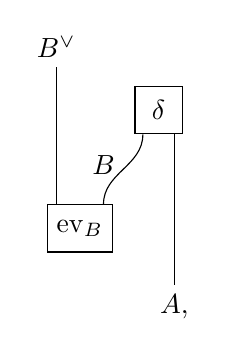
\begin{tikzpicture}[baseline=(current bounding box.center)]
      % Nodes
      \node (Bvee) at (-0.3,3.3) {$B^\vee$};
      \node (deltabox) at (1,2.5) [rectangle, draw, minimum width=0.6cm, minimum height=0.6cm] {$\delta$};
      \node (evbox) at (0,1) [rectangle, draw, minimum width=0.6cm, minimum height=0.6cm] {$\mathrm{ev}_B$};
      \node (A) at (1.2,0) {$A$,};
      \node (B) at (0.3,1.8) {$B$};

      % Edges
      \draw (Bvee) -- (evbox.north -| -0.3,1.3);
      \draw (deltabox.south -| 0.8,2.5) to [out=270,in=90] (evbox.north -| 0.3,1.3);
      \draw (deltabox.south -| 1.2,2.5) -- (A);
    \end{tikzpicture}
  \end{equation*}
  where $B^\vee = \Hom_{\mathcal C}(B,1)$ and $\mathrm{ev}_B\colon B^\vee\otimes B\to 1$ is the evaluation map, i.e. the counit of the adjunction between ${-}\otimes B$ and $\Hom_{\mathcal C}(B,{-})$.
\end{defn}
Let $\Prdual$ denote the category of dualizable stable categories with strongly continuous functors between them. The Lurie tensor product on presentable categories restricts to a symmetric monoidal structure on $\Prdual$. By \cite{Ramzi2024}, this symmetric monoidal structure is closed. We denote the resulting internal mapping object by $\Homd ({-},{-})$.
\begin{defn}[Bartels--Nikolaus]
  Let $\tset$ be a locally compact Hausdorff space. The category of \tdef{completed cosheaves} on $\tset$, denoted $\coShat (\tset )$, is given by
  \[
    \coShat (\tset ) = \Homd (\D{\tset},\Sp ).
  \]
\end{defn}
Although general objects of $\coShat (\tset )$ are quite mysterious, the definition does give us a description of the compact objects via
\[
  \coShat (\tset )^\omega\simeq\Map_{\Prdual}(\Sp ,\coShat (\tset ))
  \simeq\Map_{\Prdual}(\Sp,\Homd (\D{\tset},\Sp ))\simeq\Map_{\Prdual}(\D{\tset},\Sp),
\]
where the final equivalence used the adjunction between internal mapping object and $\otimes$. That is, the groupoid of compact objects $\coShat (\tset )^\omega$ is equivalent to the groupoid strongly continuous functors $\D{\tset}\to\Sp$, which is a subgroupoid of the more familiar groupoid of all colimit-preserving functors $\D{\tset}\to\Sp$. Of particular interest is the strongly continuous functor
\[
\tset_\sharp\colon\D{\tset}\to\Sp
\]
that is left adjoint to $\tset^*$, defined if $\tset$ is locally of singular shape. The corresponding compact object of $\coShat (\tset )$ is denoted $w_\tset$ and referred to as the \tdef{local Wall object} of $\tset$.

Another aspect of $\coShat (\tset )$ which is well-understood by hard work of Bartels--Nikolaus and Efimov is its value under localizing invariants:
\begin{thm}[Bartels--Efimov--Nikolaus]\label{thm: K theory of completed cosheaves}
  $K(\coShat (\tset ))\simeq \tset_*\tset^!K (\SS )$.
\end{thm}
Finally, we will need to introduce some notation for the functoriality of $\coShat (\tset )$. If $h\colon\tset\to\tset '$ is a proper map of locally compact Hausdorff spaces, we get as usual that the pullback $h^*\colon\D{\tset '}\to \D{\tset}$ is strongly continuous. Hence it induces a map on completed cosheaves that we denote
\[
h_?\colon \coShat (\tset )\to \coShat (\tset ').
\]
That is, the category of completed cosheaves is {\em covariantly functorial in proper maps}. Since $h_?$ is strongly continuous by construction, it admits a colimit-preserving left adjoint that we denote
\[
h^?\colon \coShat (\tset ')\to \coShat (\tset ).
\]
The reader may observe that there is an additional contravariant functoriality in etale maps, for instance, that one would might want to denote $h^{\text{?`}}$.


\medskip

Assume that $\tset$ is locally of singular shape and compact. Under these assumptions, we have a sequence of colimit-preserving functors
\[
  \D{\tset}\otimes\Sp^{\fundgroupoid (\tset )}\xrightarrow{\id\otimes\psi^*}
  \D{\tset}\otimes \D{\tset}\xrightarrow{\Delta^*}\D{\tset}\xrightarrow{\tset^*}
  \Sp, 
\]
where $\psi^*\colon \Sp^{\fundgroupoid (\tset )}\to\D{\tset}$ denotes the inclusion of local systems into all sheaves. Bartels and Nikolaus show that the composite $\D{\tset}\otimes\Sp^{\fundgroupoid (\tset )}\to\Sp$ admits a left adjoint
\[
\delta\colon \Sp\to \D{\tset}\otimes\Sp^{\fundgroupoid (\tset )},
\]
which is then a strongly continuous functor and thus a morphism in the category $\Prdual$. Specializing~\cref{defn: abstract assembly} to this situation, we thus get a strongly continuous functor
\begin{equation}
  \label{eq:BN-assembly}
  a_\delta\colon\coShat (\tset )\to \Sp^{\fundgroupoid (\tset )},
\end{equation}
the \tdef{Bartels--Nikolaus assembly functor}.
\begin{thm}[Bartels--Nikolaus]\label{thm: Bartels--Nikolaus geometric topology}
  Let $\tset$ be a compact Hausdorff space that is locally of constant shape.
  Then the functor~\eqref{eq:BN-assembly}
  \begin{enumerate}[label=(\roman*)]
  \item induces the Waldhausen assembly map on $K$-theory and
  \item maps the local Wall object $w_\tset$ to the constant sphere spectrum $\SS_{\fundgroupoid \tset}$.
  \end{enumerate}
\end{thm}
Part (ii) means that we can factor $(\fundgroupoid\tset )^*\colon\Sp\to\Sp^{\fundgroupoid\tset}$ through the Bartels--Nikolaus assembly functor. Better, we have
\begin{prop}
  Let $f\colon \tset\to \tset$ be a self-map of a compact Hausdorff space that is locally of singular shape. Considered as a morphism in $\Endtrl(\Prlstf)$, the lax commutative square~\eqref{eq:lax-comm-square-reidemeister} factors as
  \begin{equation}\label{eq:lax-composition-cosheaves}
\begin{tikzcd}
	\Sp & {\coShat(\tset)} & \Sp^{\ani{\tset}} \\
	\Sp & {\coShat(\tset)} & \Sp^{\ani{\tset}} 
	\arrow["{w_{\tset}}", from=1-1, to=1-2]
	\arrow["\id"', from=1-1, to=2-1]
	\arrow["{a_{\delta}}", from=1-2, to=1-3]
	\arrow["{f^?}", from=1-2, to=2-2]
	\arrow["f^{\ast}", from=1-3, to=2-3]
	\arrow[Rightarrow, from=2-2, to=1-3]
	\arrow["{w_{\tset}}"', from=2-1, to=2-2]
    \arrow[Rightarrow, from=2-1, to=1-2]
	\arrow["{a_{\delta}}"', from=2-2, to=2-3]
\end{tikzcd}
    % \left(
    %   \begin{tikzcd}[column sep=large]
    %     \coShat (\tset ) \arrow[r,"a_\delta"] \arrow[d,"f^?"] & \Sp^{\fundgroupoid (\tset )} \arrow[d,"f^*"]\\
    %     \coShat (\tset ) \arrow[r,swap,"a_\delta"] \arrow[ru,Rightarrow, shorten <=5pt,shorten >=5pt]  & \Sp^{\fundgroupoid (\tset )}
    %   \end{tikzcd}
    % \right)
    % \circ
    % \left(
    %   \begin{tikzcd}[column sep=large]
    %     \Sp \arrow[r,"w_\tset"] \arrow[d,equal] & \coShat (\tset ) \arrow[d,"f^?"]\\
    %     \Sp \arrow[r,swap,"w_\tset"]  \arrow[ru,Rightarrow, shorten <=5pt,shorten >=5pt]  & \coShat (\tset )
    %   \end{tikzcd}
    % \right),
  \end{equation}
  in which the left hand $2$-cell is the transpose of the commutative diagram
  \[
    \begin{tikzcd}[column sep=large]
      \coShat (\tset ) \arrow[r,"a_\delta"] \arrow[d,"f_?"] & \Sp^{\fundgroupoid (\tset )} \arrow[d,"f_!"]\\
      \coShat (\tset ) \arrow[r,swap,"a_\delta"]   & \Sp^{\fundgroupoid (\tset )}
    \end{tikzcd},
  \]
  and the right hand $2$-cell is the transpose of the $2$-cell
  \[
    \begin{tikzcd}[column sep=large]
      \Sp \arrow[r,"w_\tset"] \arrow[d,equal] & \coShat (\tset ) \arrow[d,"f_?"]\\
      \Sp \arrow[r,swap,"w_\tset"]  \arrow[ru,Leftarrow, shorten <=5pt,shorten >=5pt]  & \coShat (\tset )
    \end{tikzcd}
  \]
  coming from the counit transformation
  \[
    f_?(w_\tset) = \tset_\sharp\circ f^*\simeq\tset_\sharp \circ f_\sharp\circ f^*\to\tset_\sharp = w_\tset.
  \]
\end{prop}
\begin{cor}
  Let $f\colon \tset\to \tset$ be a self-map of a compact Hausdorff space that is locally of singular shape. There is a commutative triangle
  \begin{equation}
    \label{eq:nielsen-triangle-without-identification}
    \begin{tikzcd}[column sep=tiny]
      & \tr{f^?\curvearrowright\coShat (\tset )}{}\arrow[dr] \\
      \SS\arrow[rr]\arrow[ru] && \SS\lbrack\cL^{f}\fundgroupoid\tset\rbrack,
    \end{tikzcd}
  \end{equation}
  where the bottom horizontal arrow is the Reidemeister trace.
\end{cor}
\subsection{Another trace ``calculation''}
Keeping with the pattern laid out in~\cref{sec: lefschetz theory}, the next step in our treatment of Lefschetz--Nielsen theory is a calculation of the categorical trace that shows up as the apex in the triangle~\eqref{eq:nielsen-triangle-without-identification}. Unlike in the Lefschetz and Reidemeister trace incarnations of this step, we will not be able to calculate $\tr{f^?\curvearrowright\coShat (\tset )}{}$ in the strict sense (without a big effort); instead, we will give a lax calculation that suffices for the purposes of fixed point theory. This idea is again adapted to our setting from unpublished work of Bartels and Nikolaus, who show using simple manipulations in closed monoidal categories that the map induced on $K$-theory by their assembly functor $a_\delta\colon\coShat (\tset )\to \Sp^{\fundgroupoid (\tset )}$ factors through $\tset_*\tset^!K\SS$, thereby removing the difficult~\cref{thm: K theory of completed cosheaves} from the dependencies of the customer-facing~\cref{thm: Bartels--Nikolaus geometric topology}.

We should expect the calculation of $\tr{f^?\curvearrowright\coShat (\tset )}{}$ to be difficult, because for $f=\id$ it is already a difficult theorem of Efimov.\todo{motivate linearizing over free algebra on dualizable generator}
\begin{defn}[The free algebra on one dualizable object]
  $\freeondual = \Fun (\mathrm{Bord}^1_{\mathrm{fr}}(\RR^1)^{\op},\Sp )$\todo{define Hopf algebra structure}
\end{defn}



%We deduce a topological and homotopical Lefschetz fixed point 
via sheaves and local systems.

\subsection{Topolgical Lefschetz}

\begin{defn}
    Let $\Top$ denote the category of locally compact Hausdorff
    spaces. For any $\base \in \Top$ we write 
    $\pTop{\base} \subseteq \Top_{/\base}$ 
    for the full subcategory spanned by the proper maps $p\colon X\to \base$.
\end{defn}

Throughout this section, we make use of the following construction
from the appendix.
For any $X\in \Top$ we write $\D{X}\coloneq \Shv(X;\Sp)$ for the 
category of sheaves of spectra on $X$. Then, the assignment 
$X\mapsto \D{X}$ refines to a symmetric monoidal functor $(\infty,2)$-functor
\[ \D{-}\colon \sSpan{\pTop{\base}}_{\cP,\cI}\too \pPrlf{\base}\,.\]
Here, the source is the $(\infty,2)$-category of spans of REF and the
target is the $(\infty,2)$-category of $\D{\base}$-linear presentable
$\infty$-categories. We denote the symmetric monoidal functor underlying
$\infty$-categories
\[\cD(-)\colon \Span{\pTop{\base}}\too \pPrl{\base}\]
by the same name.
\begin{prop}
   Let $p\colon X\to \base$ be proper and let $f\colon X\to X$ be 
   a proper self map of $(X,p)$ with fixed points $i\colon X^f\to X$. 
   Then we have a map 
   \[ (pi)_!(pi)^*\SS_{X^f} \xrightarrow{\lambda^f} \SS_{\base} \in \D{\base} \]
   such that the following hold:
   \begin{enumerate}
       \item The composite $\lambda^f\epsilon$ with the unit 
       $\epsilon \colon \SS_{\base} \to (pi)_!(pi)^{\ast}\SS_{X^f}$
       is given by the
       trace of the pullback map $\pb{f}\colon p_!p^{\ast}\SS_{\base}\to p_!p^{\ast}\SS_{\base}$
       \item this identification is natural in $(\cP,\cI)$ spans.
   \end{enumerate}
\end{prop}

\appendix

\section{Trace theory}\label{sec: trace theory}
Throughout this section, fix a symmetric monoidal $(\infty,2)$-category $(\cC,\otimes)$ with
monoidal unit $\1_{\cC} \in \cC$ and write $\Omega\cC$ for the $(\infty,1)$-category of
endomorphisms $\1_{\cC} \to \1_{\cC}$. The symmetric monoidal structure on $\cC$
induces a natural symmetric monoidal structure on $\Omega \cC$, such that
the tensor product $f\otimes_{\Omega_{\cC}} g$ of two endomorphisms
$f,g\colon \1_{\cC} \to \1_{\cC}$ is simply given by the map $f\otimes g\colon \1_{\cC} \to \1_{\cC}$. 

\begin{defn}
  An object $X\in \cC$ is said to be \tdef{dualizable}
  if the functor $X\otimes - \colon \cC \to \cC$ admits an adjoint of the form
  $Y\otimes - \colon \cC \to \cC$. In this case, we write $Y= X^{\vee}$ and refer to $X^{\vee}$ as
  the \tdef{dual} of $X$. We denote by $\mdef{\cC^{\dual}}\subseteq \cC$ the full subcategory
  spanned by the dualizable objects.
\end{defn}

\begin{rmk}
  For any $X\in \cC^{\dual}$ we have a canonical equivalence $(X^{\vee})^{\vee}\simeq X$ and
  the assignment $X \mapsto X^{\vee}$ refines to an equivalence of categories
  $\cC^{\dual, \op}\rar{\sim} \cC^{\dual}$.
\end{rmk}

By definition, any $X\in \cC^{\dual}$ comes equipped with evaluation and
coevaluation maps
\[ \coev_{X}\colon \1_{\cC} \too X\otimes X^{\vee}\]
\[ \ev_{X}\colon X^{\vee} \otimes X \too \1_{\cC}\]
Moreover, since $\cC$ is symmetric monoidal, there is a canonical \textit{braiding}, giving a natural
equivalence
\[ \tau \colon X\otimes X^{\vee} \simeq X^{\vee} \otimes X \,.\]

\begin{defn}
  A \tdef{generalized endomorphism} of an object $X\in \cC$ is a map
  \[ f\colon Y\otimes X  \to X \otimes Z,\]
  for some $Y,Z\in \cC$. If $X\in \cC^{\dual}$,
  the \tdef{trace} of $f$ is defined to be the composite
  \[ \mdef{\tr{f}{\cC}} \colon  Y \rar{Y \otimes \coev_X} Y\otimes X \otimes X^{\vee} \rar{f \otimes \id} Z\otimes X \otimes X^{\vee} \rar{Z\otimes \tau} Z\otimes  X^{\vee} \otimes X \rar{Z\otimes \ev_X} Z .\]
  We refer to $\tr{\id_X}{\cC}\colon \1_{\cC} \to \1_{\cC}$ as the \tdef{dimension} of
  $X$ and denote it by $\mathrm{dim}_{\cC}(X)$.
\end{defn}

\begin{lem}\label{lem: sym mon preserve trace}
    Let $F\colon \cC\to \cD$ be a symmetric monoidal $(\infty,2)$-functor
    and let $f\colon Y\otimes X \to X\otimes Z$ be a generalized
    endomorphism of some dualizable object $X\in \cC^{\dual}$.  
    We have a natural equivalence 
    \[ F(\tr{f}{\cC})\simeq \tr{F(f)}{\cD}\,, \]
    in the $(\infty,1)$ category of maps $F(Y)\to F(Z)$. 
\end{lem}
In~\cite{Hoyois_Scherotzke_Sibilla2017} Hoyois--Scherotzke--Sibilla construct an $(\infty,1)$-category $\Endtrl(\cC)$
of \textit{traceable endomorphisms} in $\cC$ as follows:

\begin{cons}
The assignment $\cC\mapsto \cC^{\dual}$ refines to a functor
\[ (-)^{\dual}\colon \Cat^{\otimes}_{(\infty,2)} \too \Cat_{(\infty,2)}\]
which preserves filtered colimits and all limits by~\cite[Proposition 4.6.1.11]{Lurie2017}
and thus admits a left adjoint denoted by
\[ \rm{Fr}^{\dual}\colon \Cat_{(\infty,2)} \too \Cat^{\otimes}_{(\infty,2)}.\]
The $(\infty,1)$-category of traceable endomorphisms $\Endtrl(\cC)$ is defined as the maximal sub-$(\infty,1)$-category of the $(\infty,2)$-category $\Fun^{\rm{oplax}}_{\otimes}(\rm{Fr}^{\dual}(B\NN), \cC)$
of symmetric monoidal oplax functors from the ``dualizably free'' $(\infty,2)$-category
on the walking category with one endomorphism.
\end{cons}

Explicitly, objects of $\Endtrl(\cC)$ are given by self
maps of dualizable objects $f\colon X \to X$ in $\cC$, while a morphism $(X,f) \to (Y,g)$
consists of an internal left adjoint $\varphi\colon X \to Y$ together with a 2-morphism
$\alpha \colon \varphi \circ f \to g \circ \varphi $ i.e.~a lax commutative diagram
\[\begin{tikzcd}
    X & Y \\
    X & Y \arrow["\varphi", from=1-1, to=1-2] \arrow["f"', from=1-1, to=2-1] \arrow["g", from=1-2, to=2-2] \arrow["\alpha", shorten <=4pt, shorten >=4pt, Rightarrow, from=2-1, to=1-2] \arrow["\varphi"', from=2-1, to=2-2]
  \end{tikzcd}\]

\begin{thm}\cite[Theorem 1.7.]{Hoyois_Scherotzke_Sibilla2017}\label{thm: trace functor}
  The $(\infty,1)$-category $\Endtrl(\cC)$ inherits a natural
  symmetric monoidal structure, such that the assignment taking $(X,f) \in \Endtrl(\cC)$ to the
  trace $\tr{f}{\cC} \in \Omega_{\cC}$ refines to a symmetric monoidal functor
  \[ \Trc_{\cC}\colon \Endtrl(\cC) \too \Omega \cC.\]
\end{thm}

More explicitly, the functoriality of $\Trc_{\cC}$ works as follows.
Given a map $(\varphi, \alpha)\colon (X,f) \to (Y,g)$, denote by $\psi \colon Y\to X$ the internal right adjoint of $\varphi$.
Then $\Trc_{\cC}$ takes the map $(\varphi,\alpha)$ to the natural transformation given by the composite
\[ \tr{f}{\cC} \to \tr{\psi \varphi f}{\cC} \rar{\alpha} \tr{\psi g \varphi}{\cC}
\simeq \tr{\varphi \psi g}{\cC} \to \tr{g}{\cC},\]
where the first and last map are given by the unit and counit of the adjunction
$\varphi \dashv \psi$, respectively. Diagrammatically, these are also induced by the 2-cells
in the following diagram
\begin{equation}\label{eq: trace functoriality}
  \begin{tikzcd}
	{\1_\cC} & {X \otimes X^\vee} && {X\otimes X^\vee} & {\1_\cC} \\
	{\1_\cC} & {Y\otimes Y^\vee} && {Y \otimes Y^\vee} & {\1_\cC}
	\arrow["{\rm{coev}_X}", from=1-1, to=1-2]
	\arrow[equals, from=1-1, to=2-1]
	\arrow["{f\otimes \id}", from=1-2, to=1-4]
	\arrow[Rightarrow, from=1-2, to=2-1]
	\arrow["{\varphi \otimes \psi^\vee}", from=1-2, to=2-2]
	\arrow["{\ev_X}", from=1-4, to=1-5]
	\arrow["\alpha"', Rightarrow, from=1-4, to=2-2]
	\arrow["{\varphi \otimes \psi^\vee}"', from=1-4, to=2-4]
	\arrow[Rightarrow, from=1-5, to=2-4]
	\arrow[equals, from=1-5, to=2-5]
	\arrow["{\rm{coev}_Y}"', from=2-1, to=2-2]
	\arrow["{g\otimes \id}"', from=2-2, to=2-4]
	\arrow["{\ev_Y}"', from=2-4, to=2-5]
\end{tikzcd}\end{equation}

% \begin{rmk}\label{rmk:compatibility-of-fancy-trace-with-normal-trace}
%   The functor $\Trc_{\cC}$ enjoys the following compatibility with the natural symmetric
%   monoidal structure on $\Omega\cC$.
%   Given an endomorphism $\gamma \colon a \to a$ of dualizable object in $\Omega \cC$, we
%   obtain an endomorphism in $\Endtrl(\cC)$ of the form
%   \[ (a,\gamma) \colon (\1_{\cC},\id) \too (\1_{\cC},\id). \]
%   Then we have a natural equivalence
%   \[ \Trc(a,\gamma) \simeq \tr{\gamma}{\Omega \cC}\]
%   of endomorphisms of
%   $\Trc(\1_{\cC},\id)= \dim{\1_{\cC}}{\cC} = \1_{\Omega \cC} \in \Omega\cC$.\todo{Insert reference to Hoyois et al or short argument.}
% \end{rmk}

The $(-)^{\vee}\colon (\cC^{\dual})^{\op}\to \cC^{\dual}$ induces a functor on
$\Endtrl(\cC^{\dual})$ in the obvious way. Note that in general $\Endtrl(\cC)^{\dual}\neq \Endtrl(\cC^{\dual})$.

\begin{lem}
  Let $F\colon \cC\to \cD$ be a unital lax symmetric monoidal functor of symmetric monoidal $\infty$-categories. Let $X\in \cC$ be an object such that $F(X)\in \cD^{\dual}$.
  Given any $\phi \colon X^{\vee}\to Y \in \cC$ the induced map $F(\phi)\colon F(X^{\vee}) \to F(Y)$
  factors naturally through the comparison map
  \[\delta\colon F(X^{\vee})\to F(X)^{\vee}\]
  given by the adjoint of the composite 
  \[ F(X^{\vee})\otimes F(X) \to F(X^{\vee}\otimes X) \xrightarrow{F(\ev)} F(\1_{\cC})\simeq \SS.\]
\end{lem}

\begin{lem}\label{lem: trace in Span}
   Let $\cC$ be a category with finite limits and let 
   $\Lambda= (X\xleftarrow{f}Y\xrightarrow{g}Z)$ be a map
   in $\Span{\cC}$. Then we have that 
   $\tr{\Lambda}{\Span{\cC}} = (\pt \leftarrow X^{\Lambda} \to \pt ) \in \Span(\cC)$
\end{lem}

% For a map $(\varphi, \alpha)\colon (X,f) \to (X,g)$ in $\cC^{\trl}$ we refer to
% the map
% \[ \Trc(\varphi, \alpha)\colon \tr{f}{\cC} \too \tr{g}{\cC},\] obtained by
% applying $\Trc$ and using the compatibility, as the \tdef{transfer} along
% $(\varphi, \alpha)$.

% \begin{cons}\label{dim and deg}
%   Suppose we are given a map $(\varphi, \alpha)\colon (X,f) \to (X,g)$ in
%   $\cC^{\rm{trl}}$ where $f$ and $g$ are right dualizable endomorphisms of a
%   \textit{fully dualizable object} $X \in \cC$. Then by
%   Proposition~\ref{monoidal structure} the source and target are dualizable, so
%   we can form the internal trace of $(\varphi, \alpha)$ in $\cC^{\trl}$. This
%   produces an endomorphism of the unit, i.e.~a map
%   \[ (\tr{\varphi}{\cC^{\rm{trl}}},{\tr{\alpha}{\cC^{\rm{trl}}}}) \colon (\1_{\cC}, \id) \too (\1_{\cC}, \id),\]
%   which we may identify with an endomorphism
%   \[\ind{\varphi,\alpha}{}\colon \tr{\varphi}{\cC} \too \tr{\varphi}{\cC} \in \Omega\cC.\]
%   that we refer to as the \tdef{index} of $(\varphi,\alpha)$.
% \end{cons}


% \begin{prop}[Abstract Lefschetz]\label{abstract lef}
%   Let $X\in \cC$ be fully dualizable, $f,g\colon X\to X$ be two right dualizable maps and
%   $\alpha\colon fg \to gf$ be a 2-morphism considered as the data of an
%   endomorphism $(f,\alpha)\colon (X,g) \to (X,g) \in \cC$. If both $\tr{f}{\cC}$
%   and $\tr{g}{\cC}$ are dualizable in $\Omega \cC$ we have a natural equivalence
%   \[ \tr{\Trc(f,\alpha)}{\Omega \cC} \simeq \tr{\ind{f,\alpha}{}}{\Omega \cC}\]
% \end{prop}
% \begin{proof}
%   By the discussion in Remark~\ref{compatibility}, the right hand side is given
%   by taking the trace of $(f,\alpha)$ in $\cC^{\trl}$ and applying the functor
%   $\Trc$ to the resulting endomorphism of $(\1_{\cC}, \id)$. Hence, the claim follows
%   since $\Trc$ is symmetric monoidal by Theorem~\ref{trace functor} and symmetric
%   monoidal functors commute with traces.
% \end{proof}

% We also have the following symmetric statement.

% \begin{prop}[Symmetric Lefschetz]
%   Let $f,g\colon X\to X$ be right dualizable maps and let
%   $\tau\colon gf\rar{\sim} fg$ be an invertible 2-morphism.
%   If both $\tr{f}{\cC}$ and $\tr{g}{\cC}$ are dualizable in $\Omega{\cC}$ we have
%   a natural equivalence of traces of transfers
%  \[ \tr{\Trc(f,\tau)}{\Omega\cC} \simeq \tr{\Trc(g,\tau^{-1})}{\Omega\cC}.\]
% \end{prop}
% \begin{proof}
% Consider the composite $gf\colon X\to X$ together with the whiskered 2-morphism
% $\tau^{\prime}\colon gffg \rar{\sim} fggf$ as an endomorphism of $(X,fg)$ in $\cC^{\trl}$,
% diagrammatically
% given by
% \[\begin{tikzcd}
%     X & X \\
%     X & X \arrow["gf", from=1-1, to=1-2] \arrow["fg"', from=1-1, to=2-1] \arrow["fg", from=1-2, to=2-2] \arrow["{\tau^{\prime} }", shorten <=4pt, shorten >=4pt, Rightarrow, from=2-1, to=1-2] \arrow["gf"', from=2-1, to=2-2].
%   \end{tikzcd}\]
% Taking transfer and index respectively we obtain maps
% \[ \Trc(gf,\tau f) \colon \tr{f}{\cC} \too \tr{f}{\cC},\]
% \[\ind{gf,\tau f}{}\colon \tr{gf}{\cC} \too \tr{gf}{\cC}.\]
% Unwinding the definitions, we see that $\Trc(gf,\tau f) = \ind{f,\tau}{}$ and so
% by Proposition~\ref{abstract lef} twice, see that the traces of $\ind{gf}{\tau f}$,
% $\Trc(gf,\tau f)$ and $\Trc(f,\tau)$ are all canonically equivalent.
% Interchanging the roles of $f$ and $g$, we may also consider $(fg,\tau^{-1}g)$ as an
% endomorphism of $(X,g)$, obtaining maps
% \[ \Trc(fg, \tau^{-1}g):\tr{g}{\cC} \too \tr{f}{\cC}\]
% \[ \ind{fg,\tau^{-1}g}{}\colon \tr{fg}{\cC} \too \tr{fg}{\cC}.\]
% \end{proof}

% \subsection{Frobenius algebras}

% Fix $\cD\in \Pr^{\rm{rig}}$ compactly generated and denote by $\Prl_{\cD}$ the category of
% modules $\Mod_{\cD}(\Prl)$.

% \begin{defn}
%   Let $\cA\in \CAlg(\Pr_{\cD})$  be dualizable. We say that $\cA$ is
%   \begin{enumerate}
%     \item \tdef{separated} if the multiplication map
%           $\mu\colon \cA \otimes \cA \to \cA$ admits an $(\cA,\cA)$-linear internal right adjoint
%           $\delta\colon \cA \to \cA \otimes \cA$.
%     \item \tdef{prim} if the unit map $1_{\cA}\colon \cD \to \cA$ admits an
%           internal right adjoint $\eta\colon \cA \to \cD$
%     \item  \tdef{rigid} if it is separated and prim.
%     \item \tdef{co-separated} if $\mu^{\vee}\colon \cA^{\vee} \to \cA^{\vee}\otimes \cA^{\vee}$
%           admits an internal right adjoint
%     \item \tdef{suave} if $1_{\cA}^{\vee}\colon \cA^{\vee}\to \cD$ admits an internal
%           right adjoint
%     \item \tdef{co-rigid} if it is co-separated and suave.
%     \item \tdef{fully dualizable} if it satisfies all of the above.
%   \end{enumerate}
% \end{defn}

% \begin{lem}
%   Any separated $\cA$ inherits a natural \textit{Frobenius algebra} structure. In particular,
%   $\cA^{\vee}$ is also a Frobenius algebra and we have an equivalence of the underling
%   objects $\tau\colon \cA\simeq \cA^{\vee}$ that, in general, does not respect the Frobenius structures.
%   \end{lem}

% \begin{prop}
%   Let $\cA$ be rigid and suave. Then under the equivalence $\tau\colon\cA \simeq \cA^{\vee}$
%   we have that $\1_{\cA}^{\vee}\circ\tau \simeq \eta$.
% \end{prop}

% \begin{defn}
%   For any separated $\cA$ we write
%   \[ \1(\cA)\coloneq \1_{\cA}^{\vee}\circ \tau \circ\1_{\cA}\in \cD\]
%   and refer to this object as the \tdef{global sections} of $\cA$.
% \end{defn}

% Let $\cA$ be prim and suave. Then, the composite
% \[ \cD \rar{\1_{\cA}} \cA \rar{\tau} \cA^{\vee}\rar{\1_{\cA}^{\vee}} \cD \]
% defines a diagram in $(\Prlst)^{\trl}$. Applying the functor $\Trc$ to this diagram we
% get a diagram in $\cD$ of the form
% \[\begin{tikzcd}
% 	{\dim{\cA}{}} & {\dim{\cA^\vee}{}} \\
% 	\1 & \1
% 	\arrow["\sim", from=1-1, to=1-2]
% 	\arrow["{\Trc(\1_\cA^\vee)}", from=1-2, to=2-2]
% 	\arrow["{\Trc(\1_\cA)}", from=2-1, to=1-1]
% 	\arrow["{\Trc(\1(\cA))}", from=2-1, to=2-2]
% \end{tikzcd}\]


%%% Local Variables:
%%% TeX-master: "main"
%%% End:


\section{Six functor formalisms}\label{sec: verdier duality}
For the reader's convenience, we briefly review the abstract theory of six-functor formalisms following \cite{Liu_Zheng2012, Mann2022, Scholze2025, Cnossen_Lenz_Linskens2026}.

Fix a presentably symmetric monoidal $\infty$-category $\mathcal A \in \operatorname{CAlg}(\Prlst)$. We denote by $\mathrm{Pr}^{\mathrm{L}}_{\mathcal A} \coloneq \operatorname{Mod}_{\mathcal A}(\Prlst)$ the symmetric monoidal $\infty$-category of $\mathcal A$-linear presentable stable $\infty$-categories, where the monoidal product is given by the relative tensor product over $\mathcal A$. 
%Morphisms in $\mathrm{Pr}^{\mathrm{L}}_{\mathcal A}$ are colimit-preserving functors equipped with a compatible $\mathcal A$-linear structure. 

\begin{defn}\label{defn: geometric setup}
A \tdef{geometric setup} is a pair $(\mathcal C, \mathcal E)$ where $\mathcal C$ is an $\infty$-category with admits all finite limits
% \footnote{\cite{Mann2022} only asks that pullbacks along morphisms in $\mathcal E$ exist. For the sake of exposition (and because it suffices for our purposes), we require all finite limits to exist in $\mathcal C$. This also means that we do not have to mention $\infty$-operads later.}
and $\mathcal E \subseteq \Map (\mathcal C)$ is a class of morphisms
in $\cC$, satisfying the following conditions:
\begin{enumerate}[label=(\roman*)]
    \item $\mathcal E$ contains all equivalences and is closed under composition.
    \item $\mathcal E$ is stable under base change in $\mathcal C$.
\end{enumerate}
Morphisms in $\mathcal E$ are called \tdef{admissible} and we also call
an object $X\in \cC$ admissible whenever the terminal map $X\to \pt$ is.
Given a geometric setup $(\cC,\cE)$, we write $\mdef{\Span{\cC}_{\cE}}$ for the associated
symmetric monoidal $\infty$-category of \tdef{spans}, see \todo{Add Ref}. 
\end{defn}
% The pair $(\mathcal C, \mathcal E)$ determines an $\infty$-category of spans $\Span{\mathcal C}_{\mathcal E}$, which has the following informal description:
The category of spans $\Span{\cC}_{\cE}$ in a geometric
setup $(\cC,\cE)$ admits the following informal description:
\begin{itemize}
\item the objects of $\Span{\mathcal C}_{\mathcal E}$ are the same as the objects of $\mathcal C$;
\item morphisms $X\to Y$ are spans
  \[
    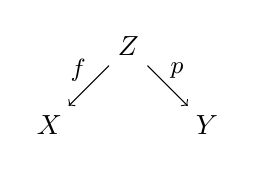
\begin{tikzpicture}[baseline=(current bounding box.center)]
      \node (X) at (-1,0){$X$};
      \node (Z) at (0,1){$Z$};
      \node (Y) at (1,0){$Y$};

      \draw (Z) edge[->] node[very near start,left=3pt]{{\small $f$}} (X);
;
      \draw (Z) edge[->] node[very near start,right=3pt]{{\small $p$}} (Y);
    \end{tikzpicture}
  \]
  with $p\in\mathcal E$; and
\item the composition of spans
    \[
      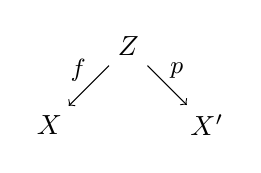
\begin{tikzpicture}[baseline=(current bounding box.center)]
        \node (X) at (-1,0){$X$};
        \node (Z) at (0,1){$Z$};
        \node (Xprime) at (1,0){$X'$};

        \draw (Z) edge[->] node[very near start,left=3pt]{{\small $f$}} (X);
        ;
        \draw (Z) edge[->] node[very near start,right=3pt]{{\small $p$}} (Xprime);
      \end{tikzpicture}
      \quad\text{and}\quad
      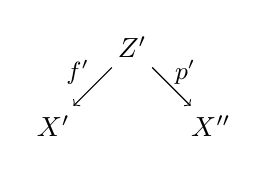
\begin{tikzpicture}[baseline=(current bounding box.center)]
        \node (X) at (-1,0){$X'$};
        \node (Z) at (0,1){$Z'$};
        \node (Xprime) at (1,0){$X''$};

        \draw (Z) edge[->] node[very near start,left=3pt]{{\small $f'$}} (X);
        ;
        \draw (Z) edge[->] node[very near start,right=3pt]{{\small $p'$}} (Xprime);
      \end{tikzpicture}
    \]
    is given by pullback---or more precisely as the outer span in the diagram
    \[
      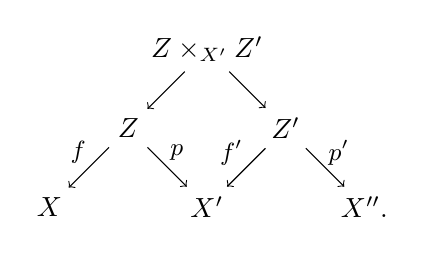
\begin{tikzpicture}[baseline=(current bounding box.center)]
        \node (X) at (-2,0){$X$};
        \node (Z) at (-1,1){$Z$};
        \node (Xprime) at (0,0){$X'$};
        \node (Zprime) at (1,1){$Z'$};
        \node (Xpprime) at (2,0){$X''.$};
        \node (pullback) at (0,2){$Z\times_{X'}Z'$};
        \node[rotate=-45] (pullbackcorner) at (0,1.6){{\large $\lrcorner$}};

        \draw (pullback) edge[->] (Z);
        \draw (pullback) edge[->] (Zprime);
        \draw (Z) edge[->] node[very near start,left=3pt]{{\small $f$}} (X);
        \draw (Z) edge[->] node[very near start,right=3pt]{{\small $p$}} (Xprime);
        \draw (Zprime) edge[->] node[very near start,left=3pt]{{\small $f'$}} (Xprime);
        \draw (Zprime) edge[->] node[very near start,right=3pt]{{\small $p'$}} (Xpprime);
      \end{tikzpicture}
    \]
\end{itemize}
Furthermore, the span category $\Span{\mathcal C}_{\mathcal E}$ has a symmetric monoidal structure, given informally by the categorical product on the underlying category $\mathcal C$. We refer to~\cites[][Definition 6.1.1]{Liu_Zheng2012}[][Definition~A.5.2 and Remark A.5.5]{Mann2022} for a precise construction of the span category and its symmetric monoidal structure.
\begin{defn}\label{defn:six-func}
  Let $(\mathcal C, \mathcal E)$ be a geometric setup and $\cA\in \CAlg(\Prlst)$ be some stable presentably monoidal category. 
  An \tdef{($\mathcal A$-linear) six-functor formalism} on 
  $(\mathcal C,\mathcal E)$ is a lax symmetric monoidal functor
  \[
    \mdef{\cD}\colon\Span{\mathcal C}_{\mathcal E}\longrightarrow
    \mathrm{Pr}^{\mathrm{L}}_{\mathcal A}.
  \]
\end{defn}
For the sake of exposition, the definition given here is more restrictive than the one in~\cite{Mann2022}, since we require $\mathcal D$ to take values in presentable categories.

\medskip

Note that any object $X\in\Span{\mathcal C}_{\mathcal E}$ has a canonical commutative algebra structure, with unit
\[
  \begin{tikzpicture}[baseline=(current bounding box.center)]
    \node (X) at (-1,0){$\pt$};
    \node (Z) at (0,1){$X$};
    \node (Xprime) at (1,0){$X$};

    \draw (Z) edge[->] (X);
    \draw (Z) edge[double equal sign distance] (Xprime);
  \end{tikzpicture}
\]
and multiplication
\[
  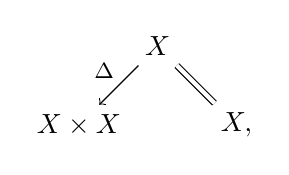
\begin{tikzpicture}[baseline=(current bounding box.center)]
    \node (X) at (-1,0){$X\times X$};
    \node (Z) at (0,1){$X$};
    \node (Xprime) at (1,0){$X,$};

    \draw (Z) edge[->] node[very near start,left=3.5pt]{{\footnotesize $\Delta$}} (X);
    \draw (Z) edge[double equal sign distance] (Xprime);
  \end{tikzpicture}
\]
see~\cite[Remark 3.13]{Scholze2025}. Unwinding the definition, we then see that a six-functor formalism on a geometric setup $(\mathcal C,\mathcal E)$ packages the following data:
\begin{itemize}
\item Since lax symmetric monoidal functors take commutative algebras to commutative algebras, we get a stable $\mathcal A$-linearly symmetric monoidal category $\mathcal D(X)\in\CAlg (\pPrl{\cA})$ for each object $X\in\mathcal C$;
\item By applying $\mathcal D$ to the span
  \[
    \begin{tikzpicture}[baseline=(current bounding box.center)]
      \node (X) at (-1,0){$X$};
      \node (Z) at (0,1){$Y$};
      \node (Xprime) at (1,0){$Y,$};

      \draw (Z) edge[->] node[very near start,left=3.5pt]{{\footnotesize $f$}}(X);
      \draw (Z) edge[double equal sign distance] (Xprime);
    \end{tikzpicture}
  \]
  we get a symmetric monoidal functor $f^*\colon \mathcal D(X)\to\mathcal D(Y)$ (called \tdef{pullback}) for each morphism $f\colon Y\to X$, together with a right adjoint $f^*\dashv f_*$ (called \tdef{pushforward});
\item By applying $\mathcal D$ to the span
  \[
    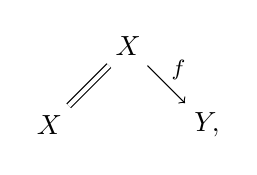
\begin{tikzpicture}[baseline=(current bounding box.center)]
      \node (X) at (-1,0){$X$};
      \node (Z) at (0,1){$X$};
      \node (Xprime) at (1,0){$Y,$};

      \draw (Z) edge[->] node[very near start,right=3.5pt]{{\footnotesize $f$}}(Xprime);
      \draw (Z) edge[double equal sign distance] (X);
    \end{tikzpicture}
  \]
  we get a functor $f_!\colon\mathcal D(Y)\to\mathcal D(X)$ (called \tdef{exceptional pushforward}) for each admissible morphism $f\colon Y\to X$ in $\mathcal C$ together with a right adjoint $f_!\dashv f^!$ (called \tdef{exceptional pullback});
\end{itemize}
Furthermore, this data satisfies
\begin{itemize}
\item \textbf{Base change:} For any cartesian square
  \[
    \begin{tikzcd}
      X' \arrow[r, "g'"] \arrow[d, "f'"] & X \arrow[d, "f"] \\
      Y' \arrow[r, "g"] & Y
    \end{tikzcd}
  \]
  in $\mathcal C$ with $f$ (and hence $f'$) admissible, 
  the Beck--Chevalley transformations $g^* f_* \xrightarrow{\sim} f'_* g'^*$ and $g_! f'^! \xrightarrow{\sim} f^! g_!$ are equivalences
\item \textbf{Projection formula:} For any admissible $f\colon Y\to X$, $A \in \mathcal D(Y)$, and $B \in \mathcal D(X)$, the canonical map $f_!(A \otimes f^* B) \to f_! A \otimes B$ is an equivalence.
\end{itemize}
\todo{Define (also for intuition of non-6FF-pilled reader): homology (ordinary and Borel--Moore), cohomology (ordinary and compactly-supported), properness, etc.}

\medskip

At first glance, it may seem that a six-functor formalism involves so much structure that it would be hard to construct one in practice. Nevertheless, \cite{Mann2022} gives a recipe (already implicit in \cite{Liu_Zheng2012}) for bootstrapping a six-functor formalism from a feasible amount of structure.\todo{This does not seem relevant to me}

Consider a geometric setup $(\mathcal C, \mathcal E)$, and suppose we are further given subclasses $\mathcal I, \mathcal P \subset \mathcal E$ such that
\begin{enumerate}[label=(\roman*)]
\item $\mathcal I$ and $\mathcal P$ contain equivalences and are under composition, base change, and diagonals.
\item If $f\in\mathcal I\cap\mathcal P$, then $f$ is $n$-truncated for some $n\geq 0$ \cite[Definition 5.5.6.8]{Lurie2009}. 
\item Every morphism $f \in \mathcal E$ admits a factorization $f = p \circ i$ with $i \in \mathcal I$ and $p \in \mathcal P$.
\end{enumerate}
Geometrically, we think of $\mathcal I$ as a class of ``open immersions'' and $\mathcal P$ as a class of ``proper maps''. Under this analogy, (ii) is then the statement that every admissible morphisms admits a compactification (cf.~Nagata compactifications in algebraic geometry, Stone--\v{C}ech compactifications in topology).
\begin{thm}[Liu--Zheng~\cite{Liu_Zheng2012}, Mann~\cite{Mann2022}]\label{thm:construction-IP}
  Let $(\mathcal C, \mathcal E)$ be a geometric setup, and let $\mathcal I$ and $\mathcal P$ be as above. Suppose we are given a functor
  \[
    \mathcal D_0\colon\mathcal C^{\mathrm{op}}\longrightarrow\CAlg (\pPrl{\cA}).
  \]
  If also
  \begin{enumerate}[label=(\roman*)]
    \setcounter{enumi}{3}
  \item the pullback $i^*$ admits a left adjoint $i_!$ for every $i\in\mathcal I$;
  \item the pushforward $f_*$ admits a right adjoint $f^!$ for every $f \in \mathcal P$; and
  \item the canonical map $i_!g_*\to f_*i'_!$ is an equivalence for every cartesian diagram
    \[
      \begin{tikzcd}
        U'\arrow[r,"i'"]\arrow[d,"g"]
        & X'\arrow[d,"f"] \\
        U\arrow[r,"i"]
        & X
      \end{tikzcd}
    \]
    in $\mathcal C$ with $f\in\mathcal P$ and $i\in\mathcal I$,
  \end{enumerate}
  then $\mathcal D_0$ admits a canonical extension to a six-functor formalism
  \[
    \mathcal D\colon\Span{\mathcal C}_{\mathcal E}\longrightarrow \pPrl{\cA}.
  \]
\end{thm}

\medskip

\todo{This is completely irrelevant}
It is often desirable to work with an $(\infty ,2)$-categorical enhancement of~\cref{defn:six-func}. Let $(\mathcal C,\mathcal E)$ be a geometric setup, and let $\mathcal I$ and $\mathcal P$ be subclasses of $\mathcal E$ satisfying conditions (i), (ii), and (iii) from the discussion preceding~\cref{thm:construction-IP}.
We can define an $(\infty ,2)$-category of spans $\sSpan{\mathcal C}_{\mathcal E,\mathcal I,\mathcal P}$ with the same objects and 1-morphisms as $\Span{\mathcal C}_{\mathcal E}$, and with 2-morphisms from $X\leftarrow Z\to Y$ to  $X\leftarrow Z'\to Y$ given by spans of spans
\[
  \begin{tikzpicture}[baseline=(current bounding box.center)]
    \node (X) at (-1.5,0){$X$};
    \node (Z) at (0,1.5){$Z$};
    \node (Zprime) at (0,-1.5){$Z',$};
    \node (W) at (0,0){$W$};
    \node (Y) at (1.5,0){$Y$};

    \draw (Z) edge[->] (Y);
    \draw (Z) edge[->] (X);
    \draw (Zprime) edge[->] (Y);
    \draw (Zprime) edge[->] (X);
    \draw (W) edge[->] node[near start,left=1.5pt]{{\footnotesize $f$}}(Z);
    \draw (W) edge[->] node[near start,left=1.5pt]{{\footnotesize $i$}}(Zprime);
  \end{tikzpicture}
\]
where $i\in\mathcal I$ and $f\in\mathcal P$. The symmetric monoidal structure on $\Span{\mathcal C}_{\mathcal E}$ extends to a symmetric monoidal structure on $\sSpan{\mathcal C}_{\mathcal E,\mathcal I,\mathcal P}$. We refer to Definition 4.10 and the discussion on page 50 in \cite{Cnossen_Lenz_Linskens2026} for the formal construction of  $\sSpan{\mathcal C}_{\mathcal E,\mathcal I,\mathcal P}$ and its symmetric monoidal structure.
\begin{thm}[Cnossen--Lenz--Linskens \cite{Cnossen_Lenz_Linskens2026}]
  Let $(\mathcal C,\mathcal E)$,$\mathcal I,\mathcal P\subseteq\mathcal E$, and $\mathcal D_0$ be as in~\cref{thm:construction-IP}. Then $\mathcal D_0$ admits a canonical extension to a lax symmetric monoidal 2-functor
  \[
    \mathcal D\colon\sSpan{\mathcal C}_{\mathcal E,\mathcal I,\mathcal P}^{\otimes}\too\mathcal P\mathrm r_{\mathcal A}^{L,\otimes_{\mathcal A}}.
  \]
\end{thm}


%%% Local Variables:
%%% mode: LaTeX
%%% TeX-master: "main"
%%% End:

%
\subsection{Verdier Duality}
Throughout this section, fix a category $\bcat$ which admits all finite limits
and a symmetric monoidal functor
\[ \D{-} \colon \Span{\bcat} \too \Prlst,\] where $\Span{\cC}$ denotes the 1-category
of spans in $\bcat$ equipped with the cartesian monoidal structure.
We write $\D{\pt}=\cD$ and note that $\D{\pt}$ refines to an object
$\D{\pt} \in \CAlg(\Prlst)$ and $\D{-}$ naturally refines to a symmetric monoidal functor
\[ \D{-} \colon \Span{\bcat} \too \Mod_{\cD}(\Prlst)\] for which we abusively use
the same notation. We also make the standing assumption that $\cD$ is compactly
generated and \tdef{rigid}, that is, an object of $\cD$ is compact if and only
if it is dualizable.
For a map $f\colon X\to Y$ in $\bcat$ we denote by
\[ f^{\ast}\colon \D{Y} \too \D{X}\] the $\D{\pt}$-linear left adjoint obtained by
applying $\D{-}$ to the span
\[\begin{tikzcd}
    & X \\
    Y && X \arrow["f"', from=1-2, to=2-1] \arrow["\id", from=1-2, to=2-3].
  \end{tikzcd}\] Conversely, we denote by
\[ f_{!}\colon \D{X} \too \D{Y}\] the $\D{\pt}$-linear left adjoint obtained by
applying $\D{-}$ to the span
\[\begin{tikzcd}
    & X \\
    X && Y \arrow["\id"', from=1-2, to=2-1] \arrow["f", from=1-2, to=2-3],
  \end{tikzcd}\] and denote the induced adjoints as
\[ f^{\ast}\dashv f_{\ast} \qquad f_{!} \dashv f^{!}.\]
\begin{defn}
  For any $X\in \bcat$ and $\cE\in \D{X}$, we write
  $\Gamma^{c}(X;\cE):=X_{!}\cE \in \D{\pt}$ and $\Gamma(X;\cE):= X_{\ast}\cE$. Moreover, for
  any map $f\colon X\to Y$ in $\bcat$ we write $\omega_{X/Y}:= f^{!}\1_{\D{Y}}$ and call
  this the \tdef{relative dualizing sheaf} of $f$. For $f=X\to \pt$, being the
  terminal map, we also write $\omega_{X}:=X^{!}\1$ and call this the (absolute)
  \tdef{dualizing sheaf} of $X$.
\end{defn}

\begin{rmk}
  The category $\D{X}$ inherits a natural presentably symmetric monoidal
  structure via the functors
  \[ X^{\ast}\colon \D{\pt} \too \D{X}\]
  \[ \Delta^{\ast}\colon \D{X \times X} \simeq \D{X} \otimes \D{X} \too \D{X}\]
\end{rmk}
Since $\D{X}$ is presentably monoidal, the functor
\[ \cE \otimes - \colon \D{X} \too \D{X},\] admits a right adjoint, which we denote by
\[ \Hom_{\D{X}}(\cE, -) \colon \D{X} \too \D{X}.\] Such that, for any $\cF\in \D{X}$ we
have an equivalence
\[ \Gamma(X;\Hom(\cE,\cF))=X_{\ast} \Hom_{\D{X}}(\cE, \cF) \simeq \map_{\D{X}}(\cE,\cF) \in \D{\pt}. \]

\begin{prop}\label{prop: projection formula}
  Let $f\colon X\to Y$ be a map in $\bcat$. Then for any $\cE, \cE^{\prime}\in \D{X}$ and
  $\cF\in \D{Y}$, we have the following natural equivalences
  \[ f_{!}(\cE \otimes f^{\ast}\cF) \simeq f_{!}(\cE)\otimes \cF\]
  \[\Hom_{\D{Y}}(f_{!}\cE, \cF)\simeq f_{\ast}\Hom_{\D{X}}(\cE, f^{!}\cF) \]
  \[ f^{!}\Hom_{\D{X}}(\cE, \cE^{\prime})\simeq \Hom_{\D{Y}}(f^{\ast}\cE, f^{!}\cE^{\prime} ).\]
\end{prop}
\begin{cons}
  Since any $X\in \Span{\bcat}$ is canonically self-dual, we also obtain a natural
  equivalence
  \[ \VD \colon \D{X} \rar{\sim} \D{X}^{\vee}, \quad \cE \mapsto X_{!}(- \otimes \cE)\] associating to
  each $\cE\in \D{X}$ the continuous functor given by the composite
  \[ \D{X} \rar{\pi_{1}^{\ast}} \D{X} \otimes \D{X} \rar{ \id \otimes \cE } \D{X} \otimes \D{X} \rar{\Delta^{\ast}} \D{X} \rar{X_{!}} \D{X}.\]
  This comes together with, for any map $f\colon X\to Y$, identifications
  \[ f^{\ast} \simeq \VD\circ~(f_{!})^{\vee}\circ \VD \]
  \[ f_{!} \simeq \VD \circ~(f^{\ast})^{\vee}\circ \VD.\] In particular, composing with the
  internal dual in $\D{X}^{\vee}$, we obtain a functor
  \[ \Dl\colon \D{X} \rar{\VD} \D{X}^{\vee} \rar{(\Hom_{\D{X}}(-,\1))^{\vee}} (\D{X}^{\vee})^{\op} \rar{ (\VD^{-1})^{\op}} \D{X}^{\op}.\]
  Unwinding the definitions, we see that $\Dl$ is given by
  \[ \Dl = \Hom_{\D{X}}(-, \omega_{X}) = \Hom_{\D{X}}(-, X^{!}\1). \]
\end{cons}

\begin{defn}
  For any $X\in \bcat$, we say that $\cE\in \D{X}$ is \tdef{reflexive}, if the
  canonical map $\Dl^{2}(\cE) \to \cE$ is an equivalence.
\end{defn}

\begin{lem}\label{lem:push pull dual}
  Let $f\colon X\to Y$ be a map in $\bcat$ and $\cE\in \D{X}$ and $\cF\in \D{Y}$. Then, we
  have natural equivalences
  \[ \Dl(f_{!}\cE)\simeq f_{\ast}\Dl(\cE) \in \D{Y}\]
  \[ f^{!}\Dl(\cF) \simeq \Dl(f^{\ast}\cF) \in \D{X}.\]
\end{lem}
\begin{proof}
  Indeed, the first equivalence is given by the composite
  \[ \Dl (f_{!}\cE) = \Hom(f_{!}\cE, \omega_{Y}) \simeq f_{\ast}\Hom(\cE, f^{!}\omega_{Y}) \simeq f_{\ast}\Hom(\cE, \omega_{X}) \simeq f_{\ast}\Dl(\cE), \]
  while the second is obtained as
  \[ f^{!}\Dl(\cF)= f^{!}\Hom(\cF, \omega_{Y}) \simeq \Hom(f^{\ast}\cE, \omega_{X}) =\Dl(f^{\ast}\cF),\]
  proving our claim.
\end{proof}

Combining the two equivalences, we learn that for a sheaf $\cF\in \D{Y}$ we have
equivalences
\[ \Gamma(X; f^{!}(\Dl(\cF)))\simeq \Gamma(X;\Dl(f^{\ast}\cF))= X_{\ast} \Dl(f^{\ast}\cF) \simeq \Dl(X_{!}f^{\ast}\cF) \simeq \Gamma^{c}(X;f^{\ast}\cF)^{\vee}.\]
In particular, for $Y=X$ and $f=\id$ we have:
\[ (X_{!}\cE)^{\vee}=\Gamma^{c}(X;\cE)^{\vee} \simeq \Gamma(X;\Dl(\cE))=X_{\ast}\Dl(\cE).\] Put
differently, this means that the functor $\D{X} \to \D{\pt}$ which takes $\cE$ to
$\Gamma^{c}(X;\cE)^{\vee}$ is represented by the dualizing sheaf $\omega_{X}$. If $X$ is
additionally assumed to be proper, i.e.~$X_{!}=X_{\ast}$, we may iterate this
reasoning to see that
\[ \Gamma(X;\Dl^{2}(\cE)) \simeq (\Gamma(X;\cE)^{\vee})^{\vee}.\]
\begin{cor}\label{cor:coherent push}
  For a proper map $f\colon X\to Y\in \bcat$, the functor $f_{!}$ preserves reflexive
  sheaves.
\end{cor}
\begin{proof}
  Since $f$ is proper, we have $f_{!}=f_{\pt}$ and so applying \cref{lem:push pull dual} twice
  we get for any reflexive $\cE\in \D{X}$ equivalences
  \[ \Dl^{2}(f_{!}\cE) \simeq \Dl(f_{!}\Dl(\cE)) \simeq f_{!}\Dl^{2}(\cE) \simeq f_{!}\cE.\]
  Thus, $f_{!}\cE\in \D{Y}$ is by definition reflexive.
\end{proof}

Notice that, for any rfelexive $\cF,\cE\in \D{X}$ we have
\[\Hom(\cF, \Dl(\cE)) \simeq \Hom(\cF \otimes \cE, \omega_{X})
  \simeq \Dl(\cF \otimes \cE).\] Replacing $\cF$ with $\Dl(\cF)$, we learn that we can
compute the internal mapping sheaf between reflexive sheaves sheaves as the tensor
product
\[ \Hom(\cF, \cE) \simeq \Hom(\cF, \Dl(\Dl(\cE))) \simeq \Dl(\cF \otimes \Dl(\cE)) \in \D{X}.\]


\begin{lem}\label{lem:suave conditions}
  Let $f\colon X\to Y$ be a proper map in $\bcat$ and let $\cE\in \D{X}$. The
  following statements are equivalent:
  \begin{enumerate}
    \item The functor $f^{\ast}(-)\otimes \cE$ has a left adjoint
    \item The functor $f_{!}(\cE \otimes -)$ has a continuous right adjoint
    \item The functor $\Hom(\cE, f^{!}(-))$ has a right adjoint
  \end{enumerate}
  Moreover, in this case we have $\Dl^{2}(\cE)\simeq \cE$ and the adjunctions are
  given by
  \[ f_{!}(\Dl(\cE)\otimes - ) \dashv f^{\ast}(-)\otimes\cE \simeq \Hom(\Dl(\cE), f^{!}(-))\] and
  \[ \Hom(\cE, f^{!}(-)) \simeq f^{\ast}(-)\otimes \Dl(\cE) \dashv f_{!}(\Dl(\cE)^{\vee} \otimes - )\]
\end{lem}
\begin{proof}
  Note that $f_{!}(\cE\otimes -)$ always admits a right adjoint given by
  $\Hom(\cE, f^{!}(-))$, so conditions (2) and (3) are clearly equivalent.
\end{proof}

\begin{defn}
  Let $f\colon X\to Y$ be a map in $\bcat$. If $\cE\in \D{X}$ satisfies any of the
  equivalent conditions of \cref{lem:suave conditions}, we call $\cE$ \tdef{$f$-suave} or just
  \tdef{suave} if $Y=\pt$ and $f$ is the terminal map. We write $\D{X}^{s}$ for the
  full subcategory of $\D{X}$ spanned by the suave sheaves on $X$. Moreover, we
  call $X\in \bcat$ suave if the unit $\1_{X}\in \D{X}$ is suave and \tdef{smooth}
  if additionally $\omega_{X}=X^{!}\1$ is dualizable.
\end{defn}

In particular, suaveness ensures that the cohomology $\Gamma(X)$ is dualizable in $\D{\pt}$.


\begin{prop}\label{prop: sections dualizable}
  Let $X\in \bcat$ be proper and $\cE\in \D{X}$ be suave. If $\1_{\cD}\in \cD^{\omega}$,
  the global sections $\Gamma(X;\cE)$ are a dualizable object of $\D{\pt}$.
\end{prop}
\begin{proof}
  Since $X$ is proper, the functor $X^{\ast}$ is strongly continuous and hence
  preserves compact objects, hence the unit $X^{\ast}\1=\1_{X}\in \D{X}$ is
  compact. Moreover, since $\cE$ is suave, the functor $X_{!}(-\otimes \cE)$
  is strongly continuous and thus $\Gamma(X;\cE)=X_{!}(\1_{X}\otimes \cE)\in \D{X}$
  is compact and hence dualizable, since $\D{\pt}$ is locally rigid..
\end{proof}

For $X\in \bcat$, denote by $\pi_{i}X\times X\to X$ the canonical projections and by
$\Delta\colon X \to X\times X$ the diagonal. The \tdef{external tensor product}
of two sheaves $\cE,\cF\in \D{X}$ is defined to be
\[ \cE\boxtimes \cF := \pi_{1}^{\ast}\cE \otimes \pi_{2}^{\ast}\cF \in \D{X\times X}.\]
Note that, we have a natural equivalence
\[ \Delta^{\ast}(\cE\boxtimes \cF)\simeq \cE\otimes \cF\in \D{X}.\]

\begin{prop}\label{prop: external hom}
Let $\cE,\cF\in \D{X}$ be suave and denote by $\pi_{i}\colon X\times X \to X$ the two projections.
Then, we have a natural equivalence
\[ \pi_{1}^{\ast}\Dl(\cE)\otimes \pi_{2}^{\ast}\cF \rar{\sim} \Hom(\pi_{1}^{\ast}\cE, \pi_{2}^{!}\cF)\in \D{X\times X}\]
\end{prop}

\begin{cor}
  If $\cE,\cF\in \D{X}$ are suave, we have a natural equivalence
  \[ \Delta^{!}(\Dl(\cE)\boxtimes \cF)\simeq\Hom(\cE, \cF) \in \D{X} .\]
\end{cor}
\begin{proof}
  Follows by applying $\Delta^{!}$ to the equivalence of \cref{prop: external hom} and
  observing that we have
  \[ \Delta^{!}\Hom(\pi_{1}^{\ast}\cE, \pi_{2}^{!}\cF)
    \simeq \Hom(\Delta^{\ast}\pi_{!}^{\ast}\cE, \Delta^{!}\pi_{2}^{!}\cF)
  \simeq \Hom(\cE, \cF)\]
by \cref{prop: projection formula} and the fact that $\pi_{i}\circ \Delta=\id$.
\end{proof}
% \end{prop}
% \begin{proof}
%   The ``if'' direction is clear by Lemma~\ref{lem:suave conditions}. For the only if direction first
%   note that $\cE$ is suave if and only if $\Dl(\cE)$ is suave. Moreover, if
%   the functor $X^{\ast}(-)\otimes \Dl(\cE)$ admits a left adjoint, it is necessarily
%   given by $X_{!}(\Dl^{2}(\cE) \otimes -)$. However, the latter functor always
%   admits a right adjoint, which is given by $\Hom(\cE,X^{!}(-))$. Since $X$ is
%   suave we have $X^{!}(-)\simeq X^{\ast}(-)\otimes \omega_{X}$ and hence $\Dl(\cE)$ is suave if
%   and only if we have an equivalence
%   \[ X^{\ast}(-)\otimes \Dl(\cE) \simeq \Hom(\cE,X^{\ast}(-)\otimes \omega_{X}) \] Since $X$ was assumed
%   to be smooth i.e.~$\omega_{X}$ is dualizable, we obtain an equivalences
%   \[ \omega_{X}\otimes \cE^{\vee}\simeq \omega_{X} \otimes \Hom(\cE, \1_{X}) \simeq \Hom(\cE, \omega_{X}) = \Dl(\cE)\]
%   as claimed.
% \end{proof}


% \begin{obs}\label{obs: diagonal comparison}
%   Let $X\in \bcat$ be separated, then there is a canonical comparison map
%   $\delta\colon \Delta^{!}\to \Delta^{\ast}$ given by the composite
%   \[ \delta\colon \Delta^{!}\simeq \Delta^{\ast}\Delta_{\ast}\Delta^{!} \simeq \Delta^{\ast}\Delta_{!}\Delta^{!}\too \Delta^{\ast},\] where the last map
%   is the unit of the adjunction $\Delta_{!}\dashv \Delta^{!}$.
% \end{obs}

% \begin{prop}
%   Let $X\in \bcat$ be separated and suave, denote the diagonal by $\Delta\colon X\to X\times X$ and
%   the two projections by $\pi_{i}\colon X\times X \to X$. For any $\cE,\cF\in \Ds{X}$, the
%   external tensor product
%   \[ \cE \boxtimes \cF:= \pi_{1}^{\ast}\cE \otimes \pi_{2}^{\ast} \cF \in \D{X\times X}\] is suave with Verdier
%   dual given by
%   \[ \Dl(\cE \boxtimes \cF)\simeq \Dl(\cE)\boxtimes \Dl(\cF)\in \D{X\times X}.\] In particular, we can
%   compute the mapping space as the exceptional inverse image
%   \[ \Hom(\cF, \cE) \simeq \Delta^{!}(\cE \boxtimes \Dl(\cF)) \in \D{X}.\]
% \end{prop}

% \begin{defn}\label{def: character}
%   Let $X$ be separated and suave. For any $\cE\in \Ds{X}$ we define the
%   \tdef{character} of $\cE$ as the composite map
%   \[ \chi^{\cE}\colon\1_{X}\rar{\id} \Hom(\cE, \cE)\simeq \Delta^{!}(\cE \boxtimes \Dl(\cE)) \rar{\delta} \Delta^{\ast}(\cE \boxtimes \Dl(\cE))\simeq \cE \otimes \Dl(\cE) \rar{\ev} \omega_{X}.\]
%   Equivalently, under the adjunction $X^{\ast}\dashv X_{\ast}$, the map $\chi^{\cE}$ defines
%   an element in the global sections $\chi^{\cE}\colon \1 \to \Gamma(X;\omega_{X})$, i.e.~a class in
%   the homology of $X$.
% \end{defn}
% \begin{prop}
%   For $X\in \bcat$ smooth with proper diagonal, the category $\Dc{X}$ inherits
%   the structure of a small, idempotent complete, stable, symmetric monoidal
%   category from $\D{X}$.
% \end{prop}
% \begin{proof}
%   Since $\Dl=\Hom_{\D{X}}(-,\omega_{X})$, the functor $\Dl^{2}$ commutes with
%   finite limits and colimits. Moreover, since any functor preserves retracts,
%   the first claim follows. Now, for any $\cE \in \D{X}^{\dual}$ we have
%   equivalences
%   \[ \Dl^{2}\cE \simeq \Dl(\Hom_{\D{X}}(\cE, \omega_{X})) \simeq \Hom_{\D{X}}(\omega_{X}\otimes \cE^{\vee},\omega_{X}) \simeq \omega_{X} \otimes (\omega_{X} \otimes \cE^{\vee})^{\vee} \simeq \cE,\]
%   and thus $\D{X}^{\dual}\subseteq \Dc{X}$, as claimed. Smallness should follows since
%   $\Dl$ induces an equivalence $\Dc{X} \simeq \Dc{X}^{\op}$ and the final claim is
%   clear since $\D{X}$ is stable and idempotent complete.
% \end{proof}
% \Fnote{The next bit is wrong cause of monoidality}

% \begin{cor}
%   Let $X\in \bcat$ be smooth and proper and let $\cE,\cF\in \D{X}$ be coherent.
%   Then $X_{!}\cE= \Gamma^{c}(X;\cE)$ and $\map(\cE ,\cF)$ are dualizable objects in
%   $\D{\pt}$.
% \end{cor}
% \begin{proof}
%   Indeed, we have that
%   \[ \map(\cE,\cF) = X_{!}\Hom(\cE,\cF)\simeq X_{!}\Dl((\cF\otimes \Dl(\cE)) = \Gamma^{c}(X;\Dl(\cF \otimes \Dl(\cE))),\]
%   and hence both claims follow from the previous lemma, using that
%   $\Dc{\pt}=\D{\pt}^{\dual}$ holds by definition.
% \end{proof}

% Let $\Cat^{\perf}_{\D{\pt}^{\dual}}$ denote the category of small, stable,
% idempotent complete, $\D{\pt}^{\dual}$-linear categories with maps given by
% exact, $\D{\pt}$-linear functors.

% \begin{prop}
%   For any smooth and proper $X\in \bcat$, the functor
%   \[ \Dc{X}^{\op} \too \Fun^{\rm{ex}}_{\Dc{\pt}}(\Dc{X},\Dc{\pt}), \quad \cE \mapsto X_{!}(\Hom(\cE, -)) \simeq X_{!}( - \otimes \Dl(\cE))\]
%   is an equivalence. Moreover, the category $\Dc{X}$ is dualizable in
%   $\Cat^{\perf}_{\D{\pt}^{\dual}}$ with dual $\Dc{X}^{\vee} = \Dc{X}^{\op}$ and
%   evaluation given by the enriched Yoneda functor
%   \[ X_{!}\Hom(-,-)\colon \Dc{X} \times \Dc{X}^{\op} \too \D{\pt}^{\dual}\] and
%   coevaluation given by the functor
%   \[ (X^{\ast}, \Dl(X^{\ast}))\colon \D{\pt}^{\dual} \too \Dc{X}\times \Dc{X}^{\op}.\]
% \end{prop}

% This allows us to fix the defect that the pullback functor $f^{\ast}$ has no
% reason to preserve coherent sheaves.
% \begin{cons}
%   Let $f\colon X\to Y \in \bcat$ be a proper map of proper, smooth spaces. We define
%   the \tdef{coherent pullback} along $f$ as the functor obtained by the
%   composition
%   \[ f^{\flat}\colon\Dc{Y} \rar{\sim} \Dc{Y}^{\vee} \rar{f_{!}^{\vee}} \Dc{X}^{\vee} \rar{\sim} \Dc{X}.\]
% \end{cons}

% \begin{defn}
%   Let $X\in \bcat$ be smooth and proper. We write $\IcD{X}$ for the Ind-category
%   of $\Dc{X}$ and call this the category of \tdef{ind-coherent} sheaves on
%   $X$.
% \end{defn}

% Write $\bcat^{sp}$ for the subcategory of $\bcat$ spanned by the smooth and
% proper objects with proper maps between them.

% \begin{prop}
%   For $X\in \bcat^{sp}$, the category $\IcD{X}$ is stable, presentable,
%   compactly generated and inherits the structure of a presentably symmetric
%   monoidal $\D{\pt}$-linear category. Moreover, $\IcD{X}$ is fully dualizable
%   and canonically self-dual.
% \end{prop}

% For $f\colon X\to Y \in \bcat^{sp}$, the functors $f^{\flat}$ and $f_{\ast}$ induce continuous
% functors on Ind-categories
% \[ f_{!}\colon \IcD{X} \too \IcD{Y} \qquad f^{\flat} \colon \IcD{Y} \too \IcD{X}.\]
% \begin{thm}
%   The functors above refine to a symmetric monoidal functor
%   \[ \IcD{-}\colon \Span{\bcat^{sp}} \too \Prlst\] i.e.~a six functor formalism.
% \end{thm}
% \subsection{Ramification}

% Let $X\in \bcat$ be a space. We want to measure ``singularities'' of $X$.

% \begin{defn}
% For a sheaf $\cE\in \D{X}$ we define its \tdef{vanishing set} to be the set of points $V(\cE)\subseteq X$
% at which the stalk $x^{\ast} \cE$ vanishes. The \tdef{support} of $\cE$ is define to be
% $S(\cE):= X\setminus V(\cE)$.
% \end{defn}

% \begin{defn}
%   We define a sheaf $\cR_{X} \in \D{X}$ called the \tdef{ramification sheaf} of $X$
%   as the fiber of the evaluation map
%   \[ \cR_{X}:= \fib \left( \omega_{X} \otimes \omega_{X}^{\vee} \too \1_{X} \right)\]
%   We say that a point $x\in X$ is \tdef{singular} if $x\in S(\cR_{X})$ and \tdef{regular}
%   else. We call $X$ regular if all of its points are regular.
% \end{defn}

% Note that $X$ is regular if and only if $\omega_{X}$ is \textit{invertible}.

% \begin{ex}
%   Let $X$ be a graph and let $x\in X$ be a point. Then the support of $\cR_{X}$ is given by those
%   vertices which have more than 2 incoming edges.
% \end{ex}

% \begin{ex}
%   Let $M$ be a manifold of dimension $n$. Then $\omega_{X}$ is locally isomorphic to the constant
%   sheaf $\S[n]$ and hence invertible, so $M$ is regular. In fact, being regular is equivalent
%   to being a homology manifold.
% \end{ex}

%%% Local Variables:
%%% TeX-master: "main"
%%% End:


%\section{Fixed point theorems}\label{sec: fixed point thms}
%\subsection{Traces in a six functor formalism}

Let $\cV$ be a stable presentably monoidal category. The category
$\Mod_{\cV}(\Prlst)$ admits a natural enhancement to a 2-category with
2-morphisms given by natural transformations of $\cV$-linear functors, such that
$\Omega \Mod_{\cV}(\Prlst)\simeq \cV$ and analogously for $\Prrst \simeq \Prlst^{\op}$.

\begin{defn}
  Let $\cV \in \CAlg(\Prl)$ and let $f\colon \cC\to \cD$ be a map of dualizable objects
  in $\Mod_{\cV}(\Prl)$. Then we write $\tr{f}{L}\in \cV$ for the trace of $f$ in
  $\Mod_{\cV}(\Prl)$. Similarly, if $g$ is the right adjoint, we write
  $\tr{g}{R}\in \cV$ for the trace in $\Mod_{\cV}(\Prr)$.
\end{defn}


\begin{defn}
  The \tdef{coincidence locus} of a pair of parallel morphisms $f,g\colon X\to Y$ in
  $\bcat$ is the pullback
  \begin{equation}
    \label{eq:coincidence}
    \begin{tikzcd}
      X^{f,g}\arrow[d]\arrow[r] & Y\arrow[d ,"\Delta"] \\
      X\arrow[r,"{(f,g)}"] & Y\times Y
    \end{tikzcd}
  \end{equation}
  If $Y = X$ and $g=\id$, we also write $X^{f} = X^{f,\id}$ and refer to this
  object as the \tdef{fixed point locus} of the map $f$.
\end{defn}
Note that, in an arbitrary category $\bcat$, the map $i\colon X^{\id} \to X$ need \textit{not}
be an equivalence.

\begin{prop}\label{trace computation}
  For any $X\in \bcat$ the category $\D{X}$ is dualizable and canonically self
  dual in $\Mod_{\D{\pt}}(\Prlst)$. Moreover, for any self map $f\colon X\to X$ there
  is a canonical equivalence
  \[
    \operatorname{tr}_{L}\left( f_{!}\colon D(X)\to D(X) \right)\simeq \Gamma^{c}(X^{f})\in \D{\pt}.
  \]
  In particular, we have $\dim{\D{X}}{L}\simeq \Gamma^{c}(X^{\id})$.
\end{prop}
\begin{proof}
  Since $D$ is symmetric monoidal, it commutes with taking trace, so we can
  instead compute the trace in the category of correspondences. The object $X$
  has a canonical self-duality given by
  $\pt\xleftarrow{p} X\xrightarrow{\Delta} X\times X$ and
  $X\times X\xleftarrow{\Delta} X\xrightarrow{p}\pt$. Thus we find that the trace is
  calculated as
  \begin{equation}\label{eq: trace span}
    \begin{tikzcd}
      &&& X^{f}\arrow[dl]\arrow[dr] \\
      && X\arrow[dl,equal]\arrow[dr,"\Delta"] && Y \arrow[dr]\arrow[dl]\\
      & X\arrow[dl,"p"] \arrow[dr,"\Delta"] && X\times X\arrow[dl,equal]\arrow[dr,"f\times\id"] && X\arrow[dl,"\Delta"] \arrow[dr,"p"] \\
      \pt & & X\times X & & X\times X & & \pt
    \end{tikzcd}
  \end{equation}
\end{proof}

Tracing through the diagram of spans, we also learn that $\Gamma^{c}(X^{f})$ is given
by the cohomology of $\Delta^{\ast}\Gamma^{f}_{!}\1_{X}= (\Gamma^{f})^{\ast}\Delta_{!}\1_{X}$, where
$\Gamma^{f}=(f\times\id)\circ \Delta$ is the \textit{graph} of $f$.

\begin{defn}\label{defn: adjectives}
  A map $f\colon X\to Y$ in $\bcat$ is called
  \begin{enumerate}
\item \tdef{suave} if $f^{\ast}$ has a left adjoint
          \item \tdef{smooth} if it is suave and $f^{!}(\1_{Y})$ is invertible
          \item \tdef{prim} if $f_{\ast}$ has a right adjoint
          \item \tdef{proper} if $f_{\ast}\simeq f_{!}$
          \item \tdef{\'etale} if $f^{\ast}\simeq f^{!}$
          \item \tdef{separated} if $\Delta_{f}\colon X\to X\times_{Y}X$ is proper
  \end{enumerate}
  If the projection $X\to \pt$ satisfies any of these properties, we also attach
  the corresponding adjective to $X$ itself.
\end{defn}

\begin{lem}
  Proper maps are closed under pullbacks.
\end{lem}

\subsection{Fixed points of proper maps}

Let $f\colon X\to Y$ be a map in $\bcat$ and suppose we are given a map of sheaves
$\sigma \colon f^{\ast}\cE \to \cF \in \D{X}$ where $\cE\in \D{Y}$ and $\cF\in \D{X}$. Then $\sigma$
induces a pullback map on cohomology
\[ \Gamma(\sigma)\colon \Gamma(Y;\cE) \too \Gamma(X;\cF) \in \D{X}\] by applying the functor $Y_{\ast}$ to the
adjoint map $\tau\colon \cE \to f_{\ast}\cF \in \D{Y}$. For $\cE= \1_{Y}$ and $\cF=\1_{X}$ and
the canonical equivalence $\sigma \colon f^{\ast}\1_{Y}\simeq \1_{X}$, the map $\Gamma(\sigma)$ is precisely
the ordinary pullback on cohomology $\Gamma(Y) \to \Gamma(X)$.\\
Let $\cC=\Mod_{\D{\pt}}(\Prlst)\in \Cat_{2}$ and let $\cC^{\trl}$ be as defined above.

\begin{defn}
  Let $f\colon X\to X$ be a self-map in $\bcat$. We define the space of
  \tdef{suave co-sheaves with $f$-transfer} to be the mapping space
  \[\D{X}_{f}:= \Map_{\cC^{\trl}}((\D{X},f_{!}), \cD).\]
\end{defn}

 Explicitly, a suave sheaf with $f$-transfer on
  $X$ is a pair $(\cE, \sigma)$ where $\cE\in \Ds{X}$ together with a
  map $\sigma \colon f^{\ast}\cE\to \cE$.

\begin{cons}
  Let $X\in \bcat$ be prim and $f\colon X\to X$ be a proper self map. Then, we have
  that $X^{\ast}\colon \D{\pt}\to \D{X}$ is an internal left adjoint and we have a natural
  transformation $\alpha\colon X^{\ast}\to f_{!}X^{\ast}$, adjoint to the equivalence
  $f^{\ast}X^{\ast}\simeq X^{\ast}$. This defines a map in $\cC^{\trl}$ of the form
  $(X^{\ast},\alpha) \colon (\D{\pt},\id) \to (\D{X},f_{!})$ and pre-composition with this
  defines a natural map
  \[ \1_{f}(X;-)\colon \D{X}_{f}\too \cL\cD;\quad
    (\cE,\sigma)\mapsto \left(\1_{f}(X;\sigma)\colon \1(X;\cE)
      \too \1(X;\cE)\right).\]
\end{cons}


\begin{cons}\label{cons:russian triangle}
  Let $X\in \bcat$ be proper, $f\colon X\to X$ a proper self map, so that
  $f^{\ast}\dashv f_{\ast}\simeq f_{!}$ and $(\cE, \sigma)$ be a suave sheaf with $f$-transfer.
  Moreover, write $\cC=\Mod_{\D{\pt}}(\Prlst) \in \Cat_{2}$. From this, we can
  form the (lax) commutative diagram in $\cC$ given by
  \[\begin{tikzcd}
      {\D{\pt}} & {\D{X}} & {\D{\pt}} \\
      {\D{\pt}} & {\D{X}} & {\D{\pt}} \arrow["{X^\ast}", from=1-1, to=1-2] \arrow[equals, from=1-1, to=2-1] \arrow["{X_!(-\otimes \cE)}", from=1-2, to=1-3] \arrow["f_{!}",from=1-2, to=2-2] \arrow[equals, from=1-3, to=2-3] \arrow["\alpha"', Rightarrow, from=2-1, to=1-2] \arrow["{X^\ast}"', from=2-1, to=2-2] \arrow["\sigma"', Rightarrow, from=2-2, to=1-3] \arrow["{X_!(-\otimes \cE)}"', from=2-2, to=2-3],
    \end{tikzcd}\]
  where the left hand transformation is adjoint to the equivalence $f^{\ast}X^{\ast}\simeq X^{\ast}$
  and the right hand transformation is given via the projection formula as
  \[ X_{!}(f_{!}(-)\otimes \cE)\simeq X_{!}f_{!}(-\otimes f^{\ast}\cE)\rar{\sigma} X_{!}(-\otimes \cE).\]
  Since $X$ is by assumption and proper and $\cE$ is suave,
  this defines a diagram in $\cC^{\trl}$
  \[ (\D{\pt},\id) \rar{(X^{\ast},\alpha)} (\D{X},f_{!}) \rar{(X_{!}(-\otimes \cE),\sigma)} (\D{\pt},\id), \]
  to which we can apply the functor $\Trc$ of \cref{trace functor} to obtain a
  commutative diagram in $\D{\pt}$
  \begin{equation}\label{eq: russian triangle}
    \begin{tikzcd}
      & {\tr{f_{!}}{L}} \\
      \1 && \1 \arrow["{\Trc(X_!(-\otimes \cE),\sigma)}", from=1-2, to=2-3] \arrow["{\Trc(X^\ast,\alpha)}", from=2-1, to=1-2] \arrow["{\Trc(X_!( X^\ast(-) \otimes \cE), \sigma\circ \alpha)}"', from=2-1, to=2-3].
    \end{tikzcd}
  \end{equation}
  We denote the map $\Trc(X_{!}(X_{!}(-\otimes \cE),\sigma))$ by
  \[ T_{(\cE,\sigma)}^{f}\colon \tr{f_{!}}{L}\simeq \Gamma^{c}(X^{f})\too \1.\] If $\cE=\1_{X}$ with
  the canonical transfer datum, we also just write $T^{f}$.
\end{cons}

Let us identify two of the maps in the diagram~\eqref{eq: russian triangle} to understand what this
means.

\begin{lem}
  In the situation of \cref{cons:russian triangle}, under the identification
  $\tr{f_{!}}{L}\simeq \Gamma^{c}(X^{f})$, the map $\Trc(X^{\ast},\alpha)$ is given by the unit
  map $\eps\colon \1 \to \Gamma^{c}(X^{f})$, i.e.~the pullback along the projection $X\to \pt$.
\end{lem}

\begin{lem}
  In the situation of \cref{cons:russian triangle}, the cohomology $\Gamma^{c}(X;\cE)$ is
  dualizable in $\D{\pt}$ and the map 
  \[\Trc(X_{!}(X^{\ast}(-)\otimes \cE), \sigma\circ \alpha)\colon \1\too \1\]
  is  given by the trace of the map
  \[\Gamma^{c}(f)\colon \Gamma^{c}(X;\cE)\to \Gamma^{c}(X;\cE)\,\in \cD.\]
\end{lem}
\begin{proof}
First note that, we are in the situation of \cref{prop: sections dualizable}, so $\Gamma^{c}(X;\cE)\in \D{X}$ is dualizable with dual given by $\Gamma(X;\Dl(\cE))$.
\end{proof}

Note that this immediately yields a general verison of the weak Lefschetz theorem.

\begin{cor}[Weak proper Lefschetz]
Let $f\colon X\to X \in \bcat$ be a proper self map of a proper and suave space $X\in \bcat$.
If $\tr{\1(f)}{\cD}$ is non-zero, then $X^{f}$ is non-empty.
\end{cor}
\begin{proof}
  By the above discussion $\tr{\1(f)}{\cD}$ factors through $\1(X^{f})\in \cD$ and so the claim
  follows since $\1(\emptyset)=0\in \cD$.
\end{proof}
% The name of the game is now to identify these maps. To this, let us give them
% names, in the hope that this grants us power over them. Note that, we can
% replace the functor $X^{\ast}$ by any internal left adjoint functor
% $E\colon\D{\ast} \to \D{X}$, together with a map $\alpha \colon E \to f_{\ast}E$, yielding a
% commutative triangle
% \[\begin{tikzcd}
%     & {\Gamma^c(X^f)} \\
%     \1 && \1 \arrow["{\Trc(X_!,\id)}", from=1-2, to=2-3] \arrow["{\Trc(E,\alpha)}", from=2-1, to=1-2] \arrow["{\Trc(X_! E, \id\circ \alpha)}"', from=2-1, to=2-3].
%   \end{tikzcd}\] We call such a pair $(E,\alpha)$ an $f$-equivariant \tdef{local
% system} on $X$ and write
% \[ \LocSys{\D{X}}{f}:= \Map_{\cC^{\trl}}(\D{\pt}, \D{X}) \] for the space of
% $f$-equivariant local systems on $X$ and write $\End(\D{\pt})$ for the space
% of pairs $(A,\varphi)$ where $A\in \D{\pt}$ and $\varphi\colon A \to A$ is an endomorphism. Then
% composition with $X_{!}$ defines a functor
% \[ \Gamma(X;-)\colon \LocSys{\D{X}}{f} \too \End(\D{\pt})\] which takes the local system
% $X^{\ast}$ with the canonical $f$-equivariant structure to the pullback map on
% cohomology
% \[ f^{\ast}\colon \Gamma^{c}(X) \too \Gamma^{c}(X).\]

% \begin{lem}
%   For any $(E,\alpha)\in \LocSys{\D{X}}{f}$ we have that the element
%   \[\Trc(X_{!}E,\id \circ \alpha) \colon \1 \too \1 \in \D{\pt}\]
%   is given by the trace of the induced map on cohomology
%   \[ f^{\ast}\colon \Gamma^{c}(X;E) \too \Gamma^{c}(X;E) \in \D{\pt}.\]
% \end{lem}

% \begin{defn}
%   Let $X\in \bcat$ be smooth and proper and $f\colon X \to X$ be a proper endomorphism.
%   Taking $(E,\alpha) \in \LocSys{\D{X}}{f}$ to the element $\1\to \Gamma^{c}(X^{f})$
%   obtained by applying the functor $\Trc$ to
%   $(E,\alpha) \colon (\D{\pt},\id) \to (\D{X},f_{\ast})$, defines a map
%   \[ \ch{f}\colon \LocSys{\D{X}}{f} \too \Omega^{\infty}\Gamma^{c}(X^{f}). \] We call
%   $\ch{f}(E) \in \Gamma^{c}(X^{f})$ the $f$-equivariant \tdef{character} of
%   $E\in \LocSys{f}{\D{X}}$.
% \end{defn}

% \begin{prop}
%   Let $(E,\alpha) \in \LocSys{\D{X}}{f}$, with $\beta\colon f^{\ast}E \to E$ being the map adjoint
%   to $\alpha$. Then, the character of $E$ is given by the trace of the induced map
%   on stalks, i.e.~we have an equivalence
%   \[ \ch{f}(E)\simeq \tr{i^{\ast} f^{\ast}E \simeq i^{\ast}E \rar{i^{\ast}\beta} i^{\ast}E}{\D{X^{f}}}\]
%   under the equivalence $\Omega^{\infty} \Gamma^{c}(X^{f})\simeq \Map_{\D{X^{f}}}(\1,\1)$, where
%   $i\colon X^{f} \to X$ is the canonical map.
% \end{prop}

% In particular, the character of a constant sheaf is trivial
% i.e.~$\ch{f}(X^{\ast}\1)$
% is given by the unit map $\1 \to \Gamma^{c}(X^{f})$.\\
Let us now turn our attention to the map $T_{f}\colon \Gamma^{c}(X^{f}) \to \1$. For
$f=\id$, this is by definition the free loop transfer along the projection map
$X\to \pt$. In general, observe that by construction of $\Trc$, the map $T_{f}$ is
given by the composite
\[ \tr{f_{\ast}}{L} \to \tr{X^{!}X_{!}f_{\ast}}{L} \simeq \tr{X^{!}X_{!}}{L} \simeq \tr{X_{!}X^{!}}{L} \to \tr{\id_{\D{\pt}}}{L}.\]
Since $X_{!}X^{!}$ is an endomorphism of the unit, we have
$\tr{X_{!}X^{!}}{L} = X_{!}X^{!}\1=\Gamma^{c}(X;\omega_{X})$ since $X$ is proper. Hence,
we obtain a canonical factorization
\[\begin{tikzcd}
    & {\Gamma^{c}(X;\omega_{X})} \\
    {\Gamma^c(X^f)} && \1 \arrow["\eta", from=1-2, to=2-3] \arrow["{\four{f}}", from=2-1, to=1-2] \arrow["{T_{f}}"', from=2-1, to=2-3],
  \end{tikzcd}\] where $\eta$ is the counit map. We call $\four{f}$ the
\tdef{$f$-equivariant Fourier transform} on $X$.

\begin{cons}
  Let $f\colon X\to X\in \bcat$ be a proper self map of a suave and proper space.
  Write $j\colon X^{f}\to X$ for the canonical map, $\Delta\colon X \to X\times X$ for the diagonal and
  $\Gamma^{f}:=(f,\id)\colon X \to X\times X$ for the graph of $f$. For a suave sheaf with transfer
  $(\cE, \sigma)$ consider the following composite:
  \begin{align*}
    \phi^{(\cE,\sigma)}\colon\Delta^{!}(\cE \boxtimes \Dl(\cE)) &\too \Delta^{!}\Gamma^{f}_{\ast}(\Gamma^{f})^{\ast}(\cE \boxtimes \Dl(\cE))\\
    &\simeq \Delta^{!}\Gamma^{f}_{\ast}(f^{\ast}\cE \otimes \Dl(\cE))\\
    &\xlongrightarrow{\sigma} \Delta^{!}\Gamma^{f}_{\ast}(\cE \otimes \Dl(\cE))\\
    &\xlongrightarrow{\ev} \Delta^{!}\Gamma^{f}_{\ast}\omega_{X}.
  \end{align*}
  By definition of $X^{f}$, we can use the Beck-Chevalley formula to see that
  $\Delta^{!}\Gamma^{f}_{\ast}\simeq j_{\ast}j^{!}$. Using this identification, we define the
  \tdef{$f$-equivariant character} of $(\cE,\sigma)$ as the composite
  \[ \chi_{f}^{(\cE,\sigma)}\colon\1_{X}\rar{\id_{\cE}}\Hom(\cE,\cE)\simeq \Delta^{!}(\cE \boxtimes \Dl(\cE)) \rar{\phi^{(\cE,\sigma)}} j_{\ast}j^{!}\omega_{X}\simeq j_{\ast}\omega_{X^{f}}.\]
  Put differently, $\ch{(\cE,\sigma)}{f}$ defines an element of
  $\1(X;j_{\ast}\omega_{X^{f}})\simeq \1(X^{f};\omega_{X^{f}})$. If $(\cE,\sigma)$ is given by $\1_{X}$ with
  the canonical transfer datum, we also just write $\ch{}{f}$.
\end{cons}

Let us unwrap this in the simplest case $\cE=\1_{X}$ with the canonical transfer
datum. We then use the equivalences
\[\1_{X}\simeq \Delta^{!}(\pi_{1}\1_{X}\otimes \pi_{2}^{\ast}\omega_{X})
  \simeq \Delta^{!}\pi_{2}^{\ast}\omega_{X}\]
and the unit transformation $\id \to \Gamma_{\ast}^{f}(\Gamma^{f})^{\ast}$ to obtain a natural
map
\[ \ch{}{f}\colon\1_{X} \too \Delta^{!}\Gamma^{f}_{\ast}(\Gamma^{f})^{\ast}\omega_{X}\simeq \Delta^{!}\Gamma^{f}_{\ast}\omega_{X}.\]

\begin{defn}\label{defn: index}
  Let $f\colon X\to X$ be a proper self map of a suave and proper space. We define
  the \tdef{fixed point index} of $f$ to be the composite
  \[ \ind{f}{}\colon \1 \rar{\ch{}{f}} \1(X^{f};\omega_{X^{f}})\rar{\eta}\1\]
\end{defn}

\begin{prop}
  Let $f\colon X\to X\in \bcat$ be a proper self map of a suave and proper space and
  let $(\cE,\sigma)\in \D{X}_{f}$. Then, under the canonical identification
  of $\1(X^{f})^{\vee}$ with $\1(X^{f};\omega_{X^{f}})$, we have that
  \[\Trc(X_{!}(- \otimes \cE), \sigma)^{\vee} \simeq \chi_{f}^{(\cE,\sigma)}\]
\end{prop}
\begin{proof}
  Apply $\D{-}$ to the trace diagram in $\Span{\bcat}$ of~\eqref{eq: trace span} and trace
  through the functoriality of trace as in~\eqref{eq: trace functoriality}.
\end{proof}

\begin{cor}[Abstract proper Lefschetz]
  Let $f\colon X\to X\in \bcat$ be a proper self map of a suave and proper space
  and let $(\cE,\sigma)\in \D{X}_{f}$. Then, we have an equivalence
  \[ \tr{\1(f,\sigma)\colon\1(X;\cE)\to \1(X;\cE)}{}
  \simeq \eta (\ch{(\cE,\sigma)}{f}) \in \1.\]
In particular, taking $\cE$ to be the unit $\1_{X}$ we obtain the formula
\[ \tr{\1(f)}{}\simeq \ind{f}{} \in \1.\]
\end{cor}

\todo{Add additive decomp for discrete spaces}

\subsection{Fixed points of \'etale maps}

Let $f\colon X\to Y\in \bcat$ be a $\cD$-\'etale map. Then, the equivalence
$f^{!}Y^{\ast}\simeq f^{\ast}Y^{\ast} \simeq X^{\ast}$ is adjoint to a map
$f_{!}X^{\ast}\to Y^{\ast}$. Hence, applying $Y_{!}$ we get a pushforward map
\[ \1(f)\colon \1(X)\too \1(Y).\]
Our goal is to show that we also obtain a Lefschetz formula for pushforward
along \'etale maps.

\begin{defn}
  Let $f\colon X\to X$ be a self map in $\bcat$. We define the space of
  \tdef{prim sheaves with $f$-transfer} on $X$ as the mapping space
  \[\D{X}^{f}:= \Map_{\cC^{\trl}}(\cD, (\D{X},f^{\ast})).\]
  If additionally, $X$ is suave and $f$ is \'etale, the functor
  $X_{!}\colon \D{X}\to \cD$ together with the natural transformation
  $X_{!}f^{\ast}\simeq X_{!}f_{!}f^{!}\to X_{!}$ obtained by applying $X_{!}$
  to the unit map $f_{!}f^{!}\to \id_{X}$ defines a map $X_{!}\colon (\D{X},f^{\ast})\to \cD$
  in $\cC^{\trl}$. We denote by
  \[ \1^{f}(X;-)\colon \D{X}^{f}\too \cL\cD^{\omega};\quad
    (\cF,\tau)\mapsto \left(\1^{f}(X;\tau)\colon \1(X;\cF)\too \1(X;\cF)\right)\]
  the map obtained by post-composition with $X_{!}$.
\end{defn}

\begin{prop}
  Let $f\colon X\to X$ be a self map and suppose that $X^{f}\in \bcat$ is either prim
  or suave and write $j\colon X^{f}\to X$ for the canonical map. Then, the assignment
  $\cE\mapsto j_{!}\cE$ induces a natural map
  \[ \D{X^{f}}\too \D{X}^{f}.\]
\end{prop}
\begin{proof}
  Consider the following pullback diagram in $\bcat$:
  \[\begin{tikzcd}
	{X^f} & {j^{-1}(X^f)} & X \\
	& {X^f} & X
	\arrow["s", from=1-1, to=1-2]
	\arrow["\id"', from=1-1, to=2-2]
	\arrow["{j^\prime}", from=1-2, to=1-3]
	\arrow["{f^\prime}"', from=1-2, to=2-2]
	\arrow["f", from=1-3, to=2-3]
	\arrow["j"', from=2-2, to=2-3].
\end{tikzcd}\]
Since $j$ is prim/suave, so are $j^{\prime}$ and $s$
\end{proof}

If $X$ is additionally prim so that $X^{\ast}\colon \cD \to \D{X}$ defines a prim sheaf
with transfer via the canonical map $\rm{can}\colon f_{!}X^{\ast} \to X^{\ast}$, then
$\1^{f}(X;\rm{can})= \1(f)$ as defined above.

\begin{defn}
  Let $f\colon X\to X$ be a self map in $\bcat$. Then applying $\Trc$ defines a natural map
  \[ \xi^{f}\colon \D{X}^{f}\too \Omega^{\infty}\1(X^{f})\in \Spc\]
  We call $\xi^{f}_{(\cF,\tau)}\colon \1 \to \1(X^{f})$ the \tdef{$f$-equivariant
  co-character} of $(\cF,\tau)$.
\end{defn}

\begin{prop}
  Let $f\colon X\to X$ be a $\cD$-\'etale self map and assume that $X$ is $\cD$-suave.
  Then the following diagram commutes
\[\begin{tikzcd}
	{\D{X}^f} & {\cL\cD^\omega} \\
	{\Omega^\infty\1(X^f)} & {\Omega^\infty\1}
	\arrow["{\1(X;-)}", from=1-1, to=1-2]
	\arrow["{\xi^f}"', from=1-1, to=2-1]
	\arrow["{\tr{-}{\cD}}", from=1-2, to=2-2]
	\arrow["\eta", from=2-1, to=2-2]
\end{tikzcd}\]
\end{prop}

\begin{proof}
  For any $(\cF,\tau) \in \pDf{X}{f}$, we get a commutative diagram:
\[\begin{tikzcd}
	{\D{\pt}} & {\D{X}} & {\D{\pt}} \\
	{\D{\pt}} & {\D{X}} & {\D{\pt}}
	\arrow["\cF", from=1-1, to=1-2]
	\arrow["\id"', from=1-1, to=2-1]
	\arrow["{X_!}", from=1-2, to=1-3]
	\arrow["{f^\ast}", from=1-2, to=2-2]
	\arrow["\id", from=1-3, to=2-3]
	\arrow["\tau"', Rightarrow, from=2-1, to=1-2]
	\arrow["\cF"', from=2-1, to=2-2]
	\arrow["\beta", Rightarrow, from=2-2, to=1-3]
	\arrow["{X_!}", from=2-2, to=2-3]
\end{tikzcd}\]
where $\beta\colon X_{!}f^{\ast}\to X_{!}$ is obtained by applying $X_{!}$ to the natural
transformation $f_{!}f^{\ast}\simeq f_{!}f^{!}\to \id_{X}$. Applying the functor $\Trc$ to this
diagram, we obtain a commutative diagram in $\cD$
\[\begin{tikzcd}
	& {\1(X^f)} \\
	\1 && \1
	\arrow["\eta", from=1-2, to=2-3]
	\arrow["{\xi^f_{(\cF,\tau)}}", from=2-1, to=1-2]
	\arrow["{\tr{\1(f,\tau)}{\cD}}"', from=2-1, to=2-3].
\end{tikzcd}\]
Unwinding the definitions, this is precisely our claim.
\end{proof}

%%% Local Variables:
%%% TeX-master: "main"
%%% End:

%\section{The topological Lefschetz fixed point theorem}\label{sec: top lefschetz}
%We now prove the thing wanted to.

\subsection{Topological Lefschetz}

Let $\bcat$ be the category of locally compact Hausdorff topological sets. Then the assignment
$X\mapsto \D{X}=\Shv(X;\Sp)$ defines a symmetric monoidal six functor formalism, \todo{Cite Marco}
which we use throughout.

\begin{lem}
  A map $f\colon X\to Y \in \bcat$ of topological sets is $\cD$-proper in the sense of~\ref{defn: adjectives} if
  and only if preimages of compact sets are compact. Moreover, if $X$ and $Y$ are compact,
  then $f$ is automatically proper.
\end{lem}

\begin{prop}
  For any $X\in \bcat$, if the projection $X\to \pt$ is a \textit{shape submersion} in the
  sense of \todo{cite} then $X$ is $\cD$-suave in the sense of~\ref{defn: adjectives}.
\end{prop}

\begin{cor}
If $X\in \bcat$ is a Euclidean neighborhood retract (ENR), e.g.~a compact CW-complex, then $X$
is $\cD$-suave.
\end{cor}

\begin{lem}
  Let $X\in \bcat$ be a compact topological manifold and let $f\colon X\to X$ be a proper
  and suave self map. Then the index of $f$ as defined in \cref{defn: index}
  agrees with the intersection number of $\Delta(X)$ and $\Gamma^{f}(X)$ in $X\times X$
  i.e.~we have
  \[ \ind{f}{}= \sharp(\Delta(X)\cap \Gamma^{f}(X))\]
\end{lem}
\begin{proof}
Follows from K-S \todo{cite}.
\end{proof}

\begin{thm}
  Let $X$ be a compact ENR and $f\colon X\to X$ be a self map such that the
  set of fixed points $X^{f}$ is finite and discrete. Then, we have an equality:
  \[ \sum_{x\in X^{f}} \ind{f}{x}= \tr{\Gamma(f)\colon \Gamma(X)\to \Gamma(X)}{\Sp}\]
\end{thm}


\subsection{Homotopical Lefschetz}

Now let $\bcat$ be the category of spaces $\Spc$. We consider the six functor formalism
given by sending $X\in \Spc$ to the category of $X$-parametrized spectra $\Sp^{X}$.

\begin{prop}
  Any map of spaces $f\colon X\to Y$ is $\cD$-\'etale. Moreover, if $f$ has compact fibers, then
  it is $\cD$-prim. In particular, any space is $\cD$-\'etale and it is $\cD$-prim
  if it is compact.
\end{prop}

\begin{prop}
  Let $f\colon X \to X$ be self map of compact space. Then, we have a natural equivalence
  \[ \tr{\S[f]\colon \S[X]\to \S[X]}{\Sp} \simeq \int_{\cL^{f} X} \xi^{f}\]
  where $\xi^{f}\colon \S\to \S[\cL^{f} X]$ is the $f$-equivariant co-character of $\S_{X}\in \Sp^{X}$.
\end{prop}

\begin{prop}
Suppose $f\colon X\to X$ is a smooth self map of a compact space. Then the
\end{prop}

% \subsection{Assembly}

% Let $X$ be a compact $CW$-complex considered as a static condensed space and let $f\colon X\to X$
% be self-map. Then $X$ has an associated discrete space $\ani{X}\in \CondSpc$, together
% with a comparison map
% \[ \as \colon X\too \ani{X}\in \CondSpc.\]
% Moreover, $f$ induces a map $\abs{f}\colon \abs{X}\to \abs{X}$ of the associated spaces,
% fitting into a diagram
% \[\begin{tikzcd}
% 	X & X \\
% 	{\abs{X}} & {\abs{X}}
% 	\arrow["f", from=1-1, to=1-2]
% 	\arrow["\as",from=1-1, to=2-1]
% 	\arrow["\as",from=1-2, to=2-2]
% 	\arrow["{\abs{f}}", from=2-1, to=2-2].
% \end{tikzcd}\]

% \begin{defn}
%   We say that $X\in \CondSpc$ is homotopical if the shape of $X$ is pro-constant and denote the
%   associated discrete space by $\ani{X}\in \CondSpc$.
% \end{defn}

% \begin{prop}
%   Let $X\in \CondSpc$ be homotopical. If $X$ is suave, then the map $\as\colon X\to \ani{X}$
%   is suave.
% \end{prop}

% \begin{lem}
%   For any locally compact Hausdorff space $X$, the functor
%   \[\as^{\ast}\colon \D{\abs{X}}\too \D{X}\]
%   is fully faithful with essential image given by the locally constant sheaves on $X$.
% \end{lem}

% \begin{cons}
%   Let $X\in \CondSpc$ be homotopical, suave an prim. Then the comparison map $\as \colon X \to \ani{X}$ is suave as well, and hence $\as^{\ast}$ admits a left adjoint $\as_{\sharp}$.
%   Consider the following composite in $\Prlst$:
%   \[ \Sp \rar{X^{\ast}} \D{X} \rar{\as_{\sharp}} \D{\ani{X}} \rar{\ani{X}_{!}} \Sp.\]
%   Since $X$ is prime, $X^{\ast}$ is strongly continuous and $\ani{X}$ is \'etale \todo{Really?}.
%   Hence, all functors are strongly continuous and we may apply $\Trc$ to obtain a
%   commutative diagram
%   \[\begin{tikzcd}
% 	{\S(X)} && {\S[\cL \ani{X}]} \\
% 	\S && \S
% 	\arrow["{\Trc(\as_{\sharp})}", from=1-1, to=1-3]
% 	\arrow[from=1-3, to=2-3]
% 	\arrow[from=2-1, to=1-1]
% 	\arrow["{\Trc(\ani{X}_!(\as_\sharp\S_X))}", from=2-1, to=2-3].
% \end{tikzcd}\]
% Note that, since $\ani{X}$ is \'etale we have
% \(\abs{X}_{!}\as_{\sharp}\simeq X_{\sharp}\simeq X_{!}(-\otimes \omega_{X})\). In particular, we learn that we get a factorization
% \[\begin{tikzcd}
% 	& {\S[\cL\ani{X}]} \\
% 	{\S(X)} & \S
% 	\arrow[from=1-2, to=2-2]
% 	\arrow["{\Trc(\as_\sharp)}", from=2-1, to=1-2]
% 	\arrow["T"', from=2-1, to=2-2]
% \end{tikzcd}\]
% \end{cons}


% Now $X$ is suave and $f$ is proper. Moreover, $\abs{X}$ is compact, hence prim and \'etale
% and $\abs{f}$ is \'etale. Thus, applying our constructions, we get both a ``topological'' character
% \[ \chi_{f}\colon \S \too \Gamma^{c}(X^{f},\omega_{X})\]
% and a ``homotopical'' character map
% \[ \xi^{f}\colon \S \too \S[\cL^{f}\abs{X}],\]
% where we have written $\abs{X}^{f}=\cL^{f}\abs{X}$ for emphasis.
% Post-composing with the projection maps, we learn that
% \[ \int_{X^{f}}\chi_{f}=  \tr{\Gamma^{c}(f;\omega_{X})}{\Sp} \simeq \tr{\S[f]}{\Sp}
%   \simeq \int_{\abs{X}^{f}}\xi^{f}\in \S.\]

% \begin{prop}
%   The canonical comparison map $c\colon X\to\ani{X}$ induces a commutative diagram
% \[\begin{tikzcd}
% 	{\S[\cL^f\ani{X}]} & {\Gamma^c(X^{f};\omega_X)} \\
% 	\S & \S
% 	\arrow[from=1-1, to=1-2]
% 	\arrow["{\xi^f}"', from=2-1, to=1-1]
% 	\arrow[from=2-1, to=2-2]
% 	\arrow["{\chi_f}", from=2-2, to=1-2]
% \end{tikzcd}\]
% \end{prop}
\section{Actions of cyclic groups}
Let $p$ be a prime and write $C_{p}$ for the cyclic group with $p$-elements. If $X$ is a compact
Hausdorff space, then a $C_{p}$-action on $X$ is the same as a continuous self-map $f\colon X\to X$
satisfying $f^{p}= \id$. The idea is that this ``untwists'' the $f$-equivariant character
of $\S_{X}$.

\begin{thm}
  Let $X$ be an $\F_{p}$-finite $p$-complete space and let $G$ be a cyclic $p$-group. Then,
  for any generator $g\in G$, we have that
  \[ \chi(X^{hG})= \tr{\S[g]\colon \S[X]\to \S[X]}{}.\]
\end{thm}

Classically: The trace of an idempotent is given by the rank.
This should mean for us
$\tr{\S[g]}{} = \chi(X) - \dim{\fib(g)}{}$ or something.\\

Noting that $\cL^{g}X= X^{h\ZZ}$ where $\ZZ$ acts via $g$, we see that
it will suffice to show the following:
\begin{prop}
The canonical map $X^{hG}\to X^{h\ZZ}$ induces a commutative diagram
\[\begin{tikzcd}
	\S & {\S[X^{hG}]} & {} \\
	\S & {\S[\cL^gX]}
	\arrow["\chi", from=1-1, to=1-2]
	\arrow["\id"', from=1-1, to=2-1]
	\arrow[from=1-2, to=2-2]
	\arrow["{\xi^g}", from=2-1, to=2-2]
\end{tikzcd}\]
\todo{Unclear if this is true}
\end{prop}


%%% Local Variables:
%%% TeX-master: "main"
%%% End:

\printbibliography{}

\end{document}

%%% Local Variables:
%%% mode: LaTeX
%%% TeX-master: t
%%% End:
